
\chapter{Heat and Salt fluxes}
\label{ch:heatsaltflux}
% \section{Introduction}

The ocean is moved by three main forcings - friction from the winds, body forces due to astronomical forcing i.e. the tides, and differences in buoyancy forcing.  This section discusses the buoyancy forcing.  The buoyancy of water is how dense it is, and as we saw in the previous chapter, it is determined by the temperature of the water and how much salt it has in it (and of course the pressure).  

This is crucially important for the circulation of the ocean.  We already saw how estuaries have differential buoyancy forcing due to a freshwater source at the head of the estuary being more buoyant than the salty ocean water.  Buoyancy forcing by fresh water is also important on a global scale.  Perhaps even more important is the differential heating, with the ocean gaining heat near the equator and losing it near the poles.  This transport of heat is approximately 30\% of the poleward transport of heat, the rest is done by the atmosphere.  However, it also drives the overturning circulation of the global ocean. 

Like an estuary, if the ocean only had heating and cooling at the surface the total volume transport of water in the overturning circulation would be weak.  However, mixing brings heat to great depths in the ocean and this creates pressure gradients that move a large slow overturning.


\section{Surface heat fluxes}

Most heat exchange in the ocean occurs at the surface, with short wave radiation passing through the atmosphere and impacting the ocean, and then the ocean losing heat to back radiation, latent heat flux, and heating and cooling from direct contact with the atmosphere.


An estimate of the net heat flux in the ocean is given in \fref{fig:SurfaceHeatFluxes}e.  Recall that heat is specified in units of Joules, where 1 Joule is the energy (or heat) required to warm a kilogram of water one degree Kelvin.  Heat fluxes are a rate of heating, and hence are in units of Watts, or Joules per second.  If we want to make a map like \fref{fig:SurfaceHeatFluxes}e, then we want to know the rate of heating per area, and we plot in units of Watts per meter squared, or $\mathrm{W\,m^{-2}}$.  One thing to keep in mind when looking at figures like \fref{fig:SurfaceHeatFluxes} is that this is a projection of a sphere, and that the polar regions have much less area than the equatorial ones.  

\subsection{Incoming shortwave radiation}

The spatial distribution of these fluxes and their net magnitudes indicate that, unsurprisingly, the net incoming shortwave radiation is strongest at the equator (\fref{fig:SurfaceHeatFluxes}a).  This radiation comes from the sun, and is modified as it passes through the atmosphere.  Of course it includes all wavelengths of radiation, but it is very much dominated by short scale radiation, so it is called "shortwave".  

Estimating the radiation coming from the sun and impacting the ocean would be a simple matter depending only on the tilt of the earth, and to a (much) lesser extent whether the sun is in aphelion or perihelion.  However, the atmosphere severely modifies the net flux reaching the earth, due to ozone and clouds.  Indeed, much of the east-west spatial variability to the shortwave surface fluxes is due to clouds. For instance, the inter-tropical convergence zone can be clearly seen just north of the equator (\fref{fig:SurfaceHeatFluxes}a) as a region of reduced incoming radiation.  

\begin{figure}[htb]
  \centering
  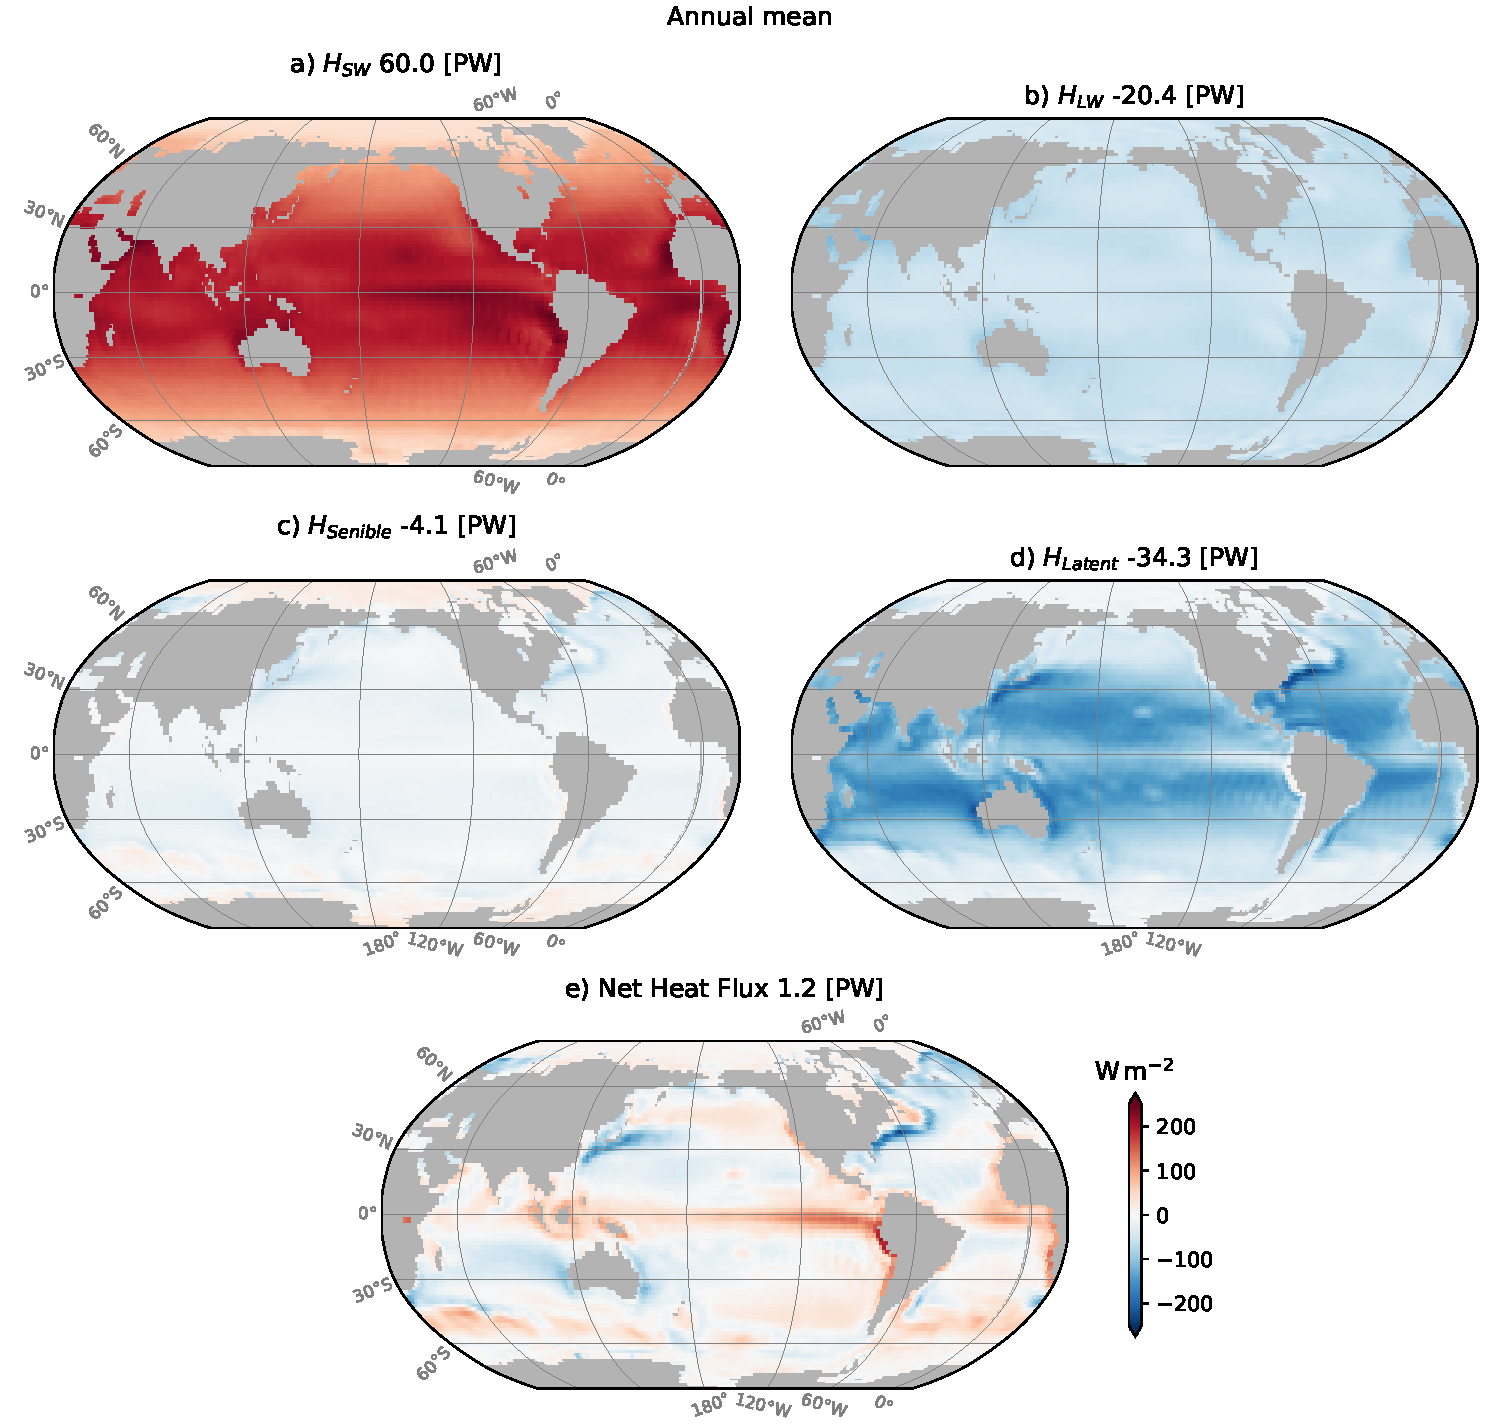
\includegraphics[width=4.5in]{FluxesFigs/SurfaceHeatFluxes}
  \caption{Net surface heat fluxes, annually averaged.  a) Net shortwave heat flux, b) net longwave flux, c) sensible heat flux, d) latent heat flux and e) net heat flux. 
  Data source:  \href{https://psl.noaa.gov/data/gridded/data.ncep.reanalysis.derived.surfaceflux.html}{NCEP1 reanalysis.}  }
  \label{fig:SurfaceHeatFluxes}
\end{figure}

Given this, it is important to realize that it is very difficult to make accurate estimates of the incoming radiation over the full expanse of the ocean.  Satellites make this easier, because they give a good idea of cloud cover, but the thickness of the clouds and their humidity all matter to making an estimate.  Radiation can be measured with \href{https://en.wikipedia.org/wiki/Radiometer}{radiometers}, but these need ships, moorings, or other platforms to make direct measurements. Hence estimates of shortwave radiation are derived from empirical models.  

Some idea of the magnitude of the problem can be seen by considering the net heat flux of 1.2 PW (\fref{fig:SurfaceHeatFluxes}e) integrated over the entire global ocean (1 PW is $10^{15}\ \mathrm{Watts}$). The volume of the oceans is approximately $1.335\times10^{18}\ \mathrm{m^3}$. The heat capacity of water is $4180 \mathrm{J\, kg^{-1}}$ and its density approximately $1030 \ \mathrm{kg\,m^{-3}}$.  Using these numbers, this 1.2 PW discrepency in the annual mean would lead to a one-degree warming of the ocean over 140 years.  This would be quite large and rapid, even on the scale of anthropogenic climate change, and this net should be considered a bound on how accurate the various terms of the budget are, rather than a direct estimate of how fast the ocean is warming.  

\begin{figure}[htb]
  \centering
  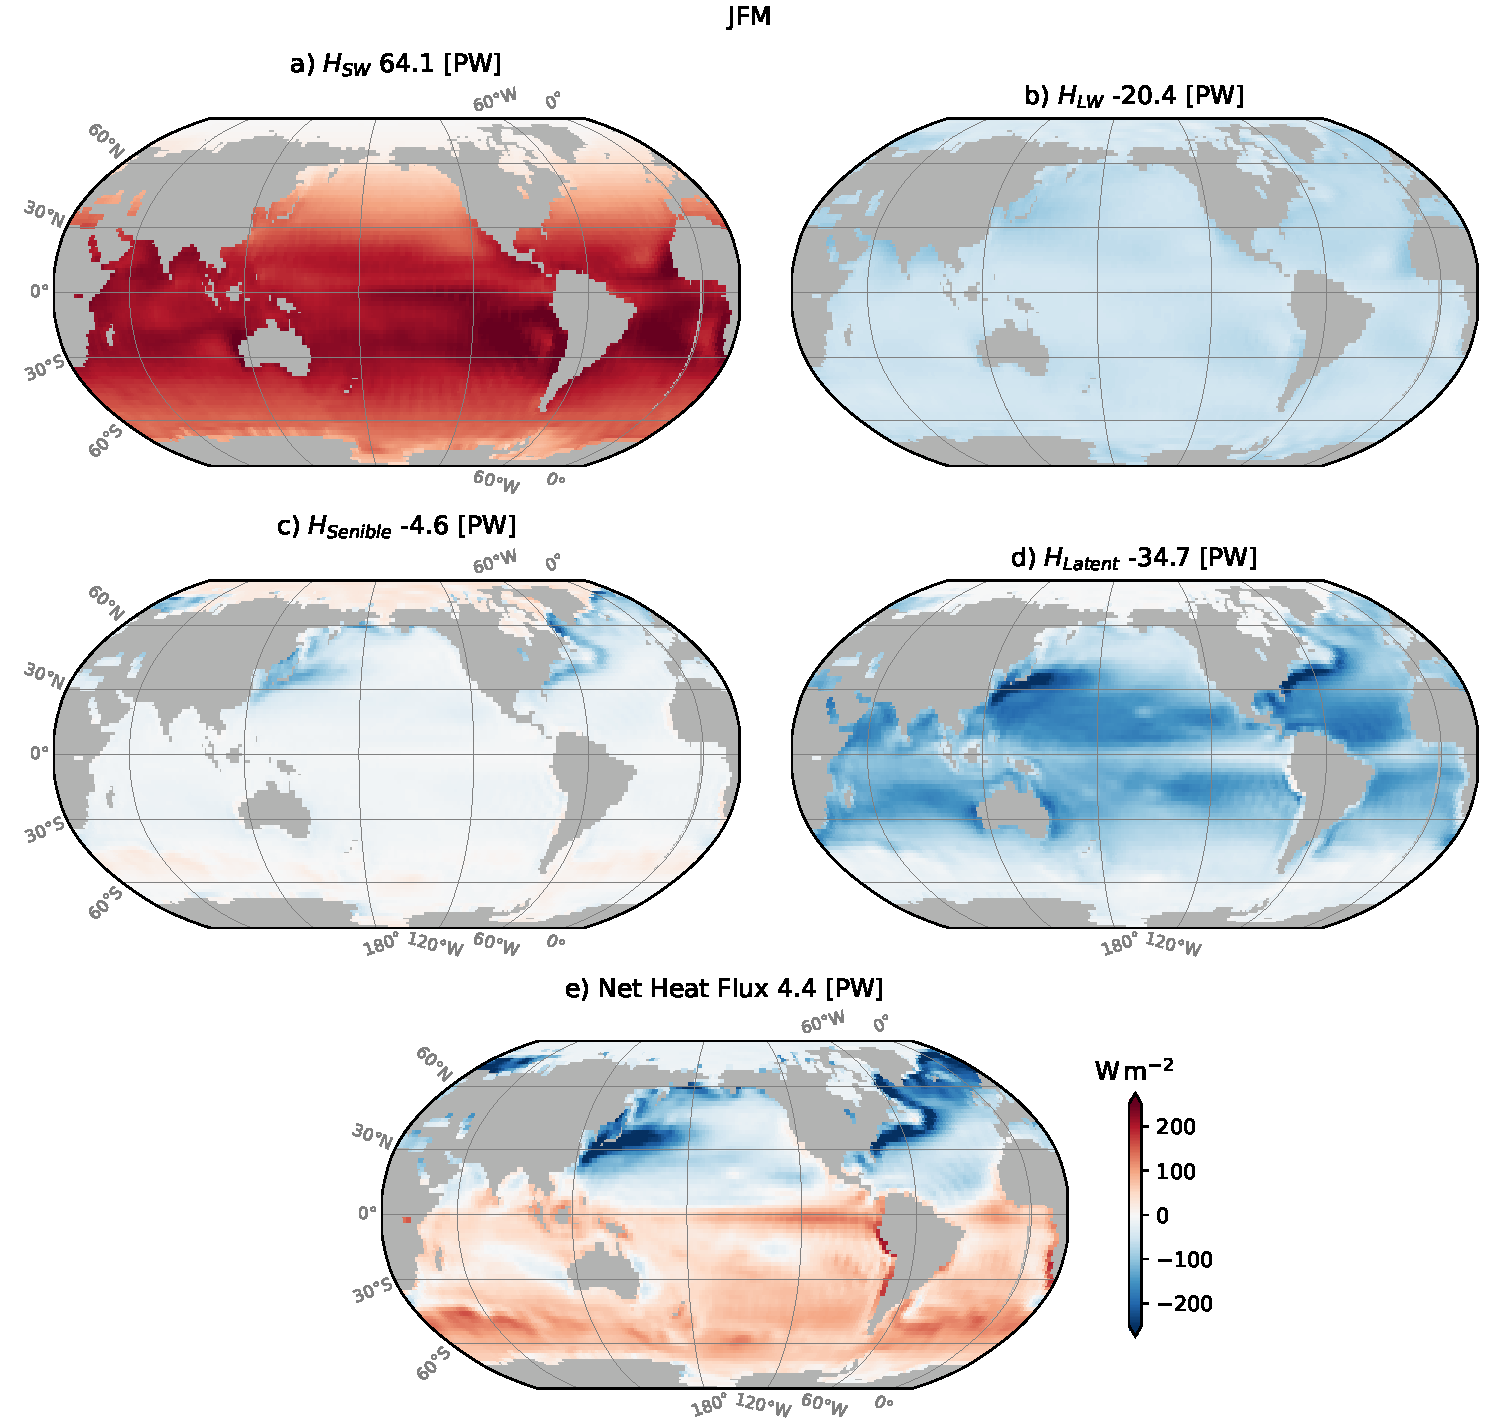
\includegraphics[width=4.5in]{FluxesFigs/SurfaceHeatFluxesJFM}
  \caption{Net surface heat fluxes, January to March.  a) Net shortwave heat flux, b) net longwave flux, c) sensible heat flux, d) latent heat flux and e) net heat flux. 
  Data source:  \href{https://psl.noaa.gov/data/gridded/data.ncep.reanalysis.derived.surfaceflux.html}{NCEP1 reanalysis.}  }
  \label{fig:SurfaceHeatFluxesJFM}
\end{figure}

We can see the effect of the earth's tilt and changing cloud cover if we look at seasonal averages of the shortwave radiation (\fref{fig:SurfaceHeatFluxesJFM}a, \fref{fig:SurfaceHeatFluxesAMJ}a, \fref{fig:SurfaceHeatFluxesJAS}a, \fref{fig:SurfaceHeatFluxesOND}a).  Not surprisingly, during the boreal winter, the net radiation is low in the northern hemisphere, than in the boreal summer.  

\begin{figure}[htb]
  \centering
  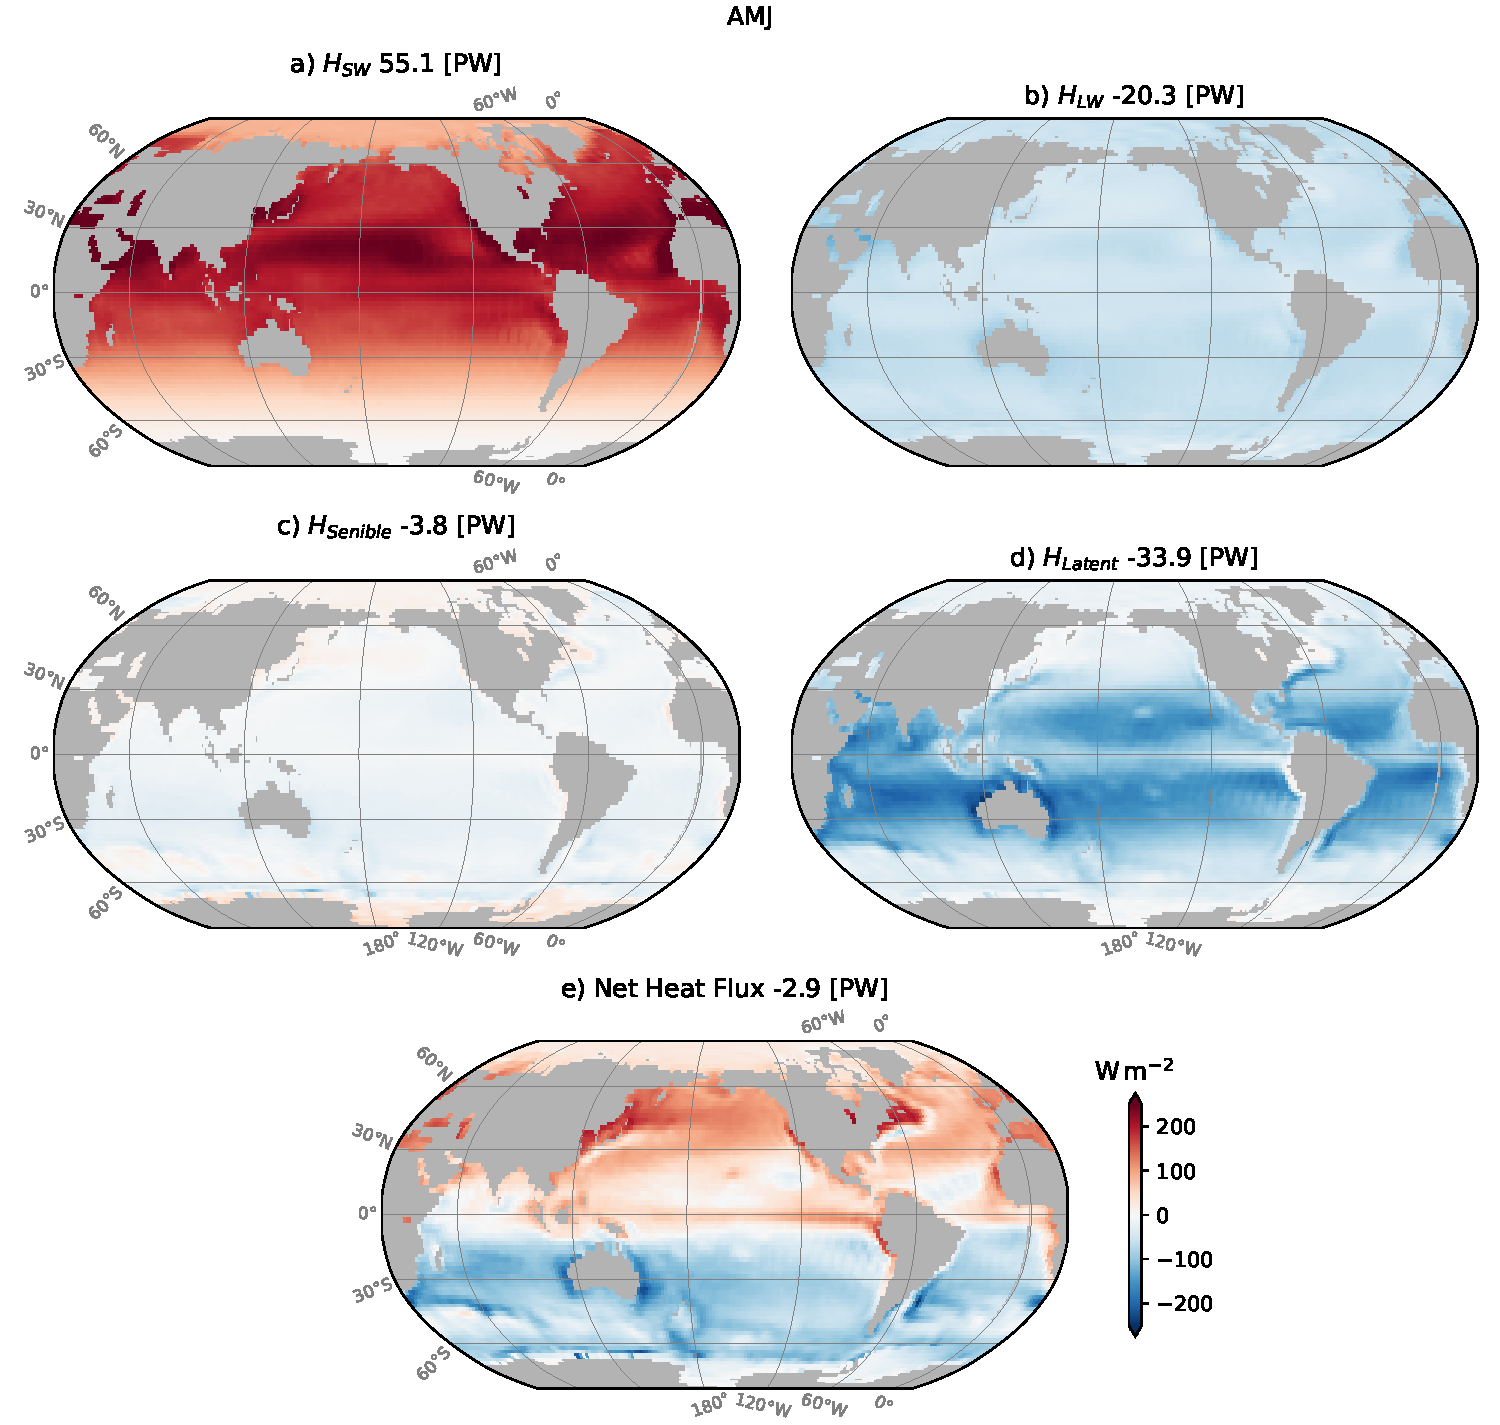
\includegraphics[width=4.5in]{FluxesFigs/SurfaceHeatFluxesAMJ}
  \caption{Net surface heat fluxes, April to June.  a) Net shortwave heat flux, b) net longwave flux, c) sensible heat flux, d) latent heat flux and e) net heat flux. 
  Data source:  \href{https://psl.noaa.gov/data/gridded/data.ncep.reanalysis.derived.surfaceflux.html}{NCEP1 reanalysis.}  }
  \label{fig:SurfaceHeatFluxesAMJ}
\end{figure}

\begin{figure}[htb]
  \centering
  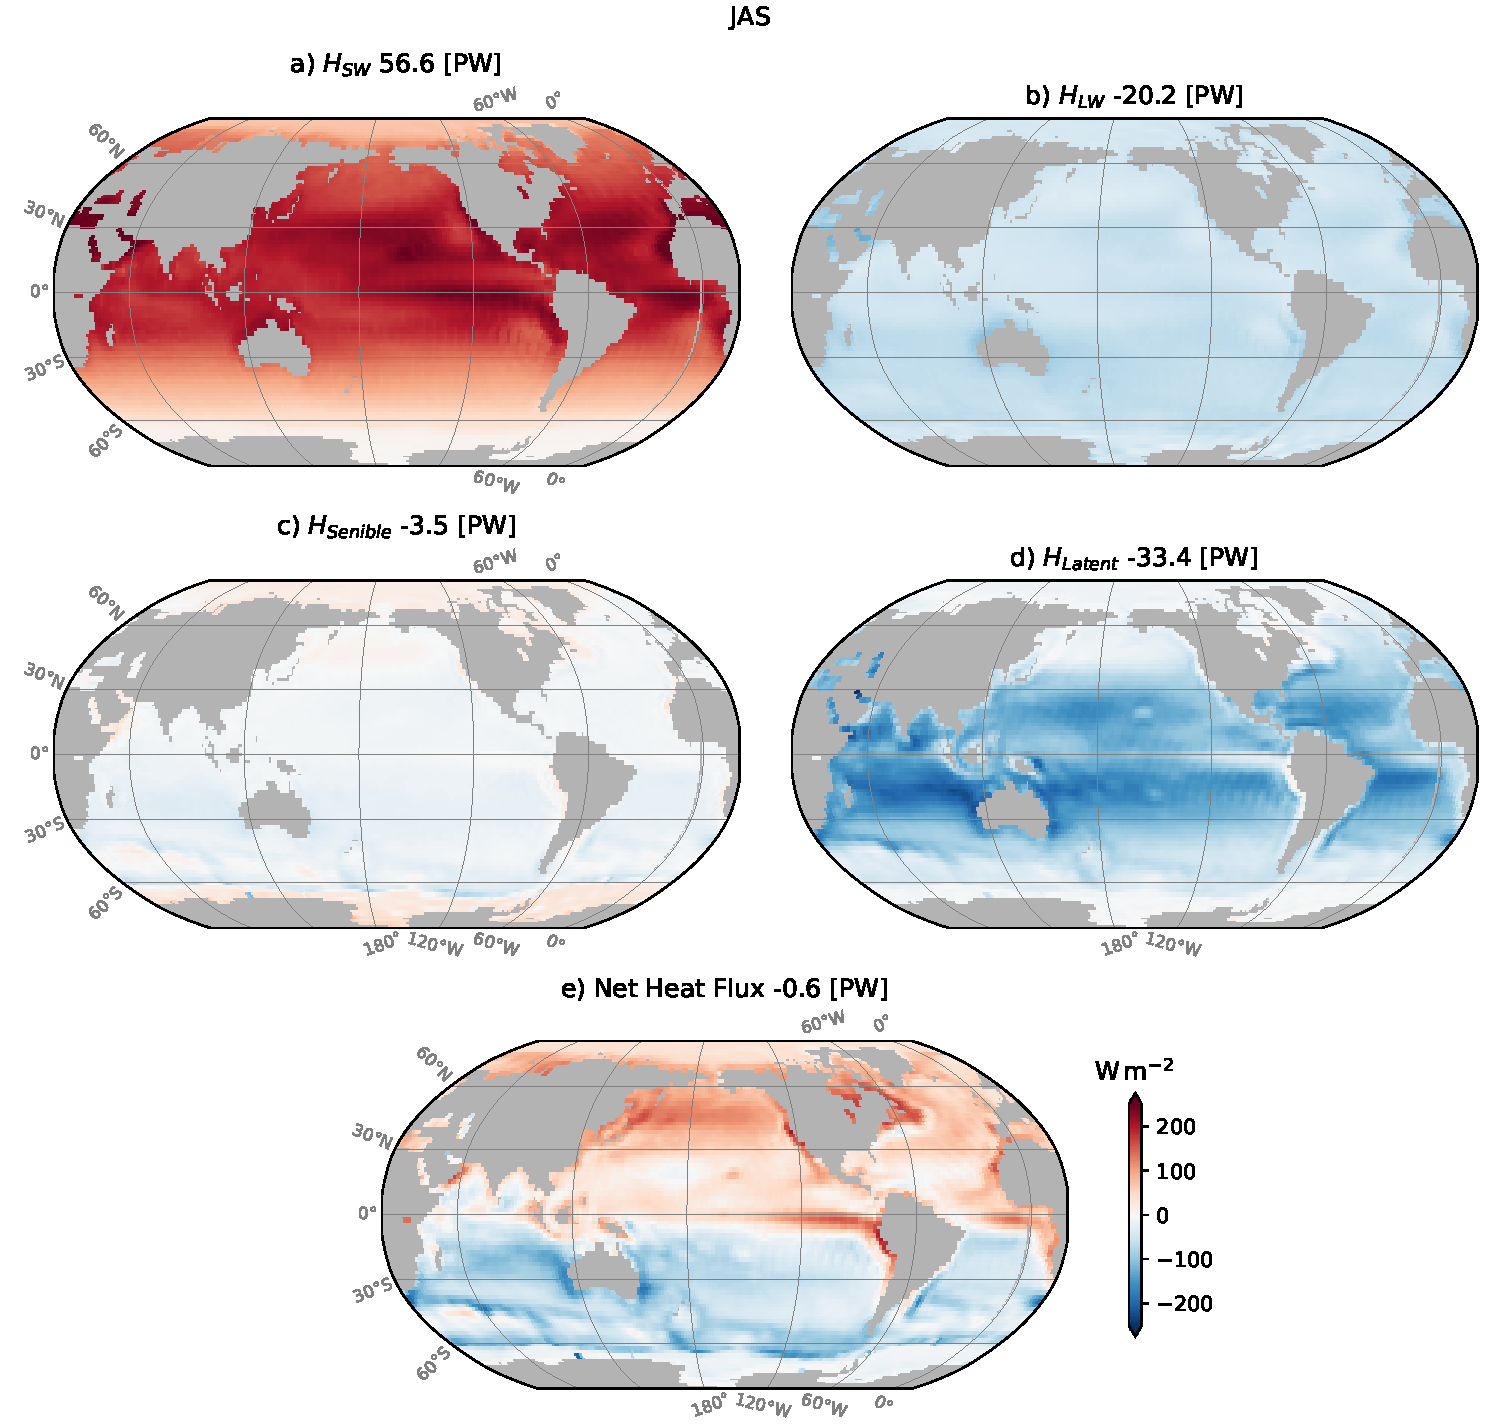
\includegraphics[width=4.5in]{FluxesFigs/SurfaceHeatFluxesJAS}
  \caption{Net surface heat fluxes, July to September.  a) Net shortwave heat flux, b) net longwave flux, c) sensible heat flux, d) latent heat flux and e) net heat flux. 
  Data source:  \href{https://psl.noaa.gov/data/gridded/data.ncep.reanalysis.derived.surfaceflux.html}{NCEP1 reanalysis.}  }
  \label{fig:SurfaceHeatFluxesJAS}
\end{figure}

\begin{figure}[htb]
  \centering
  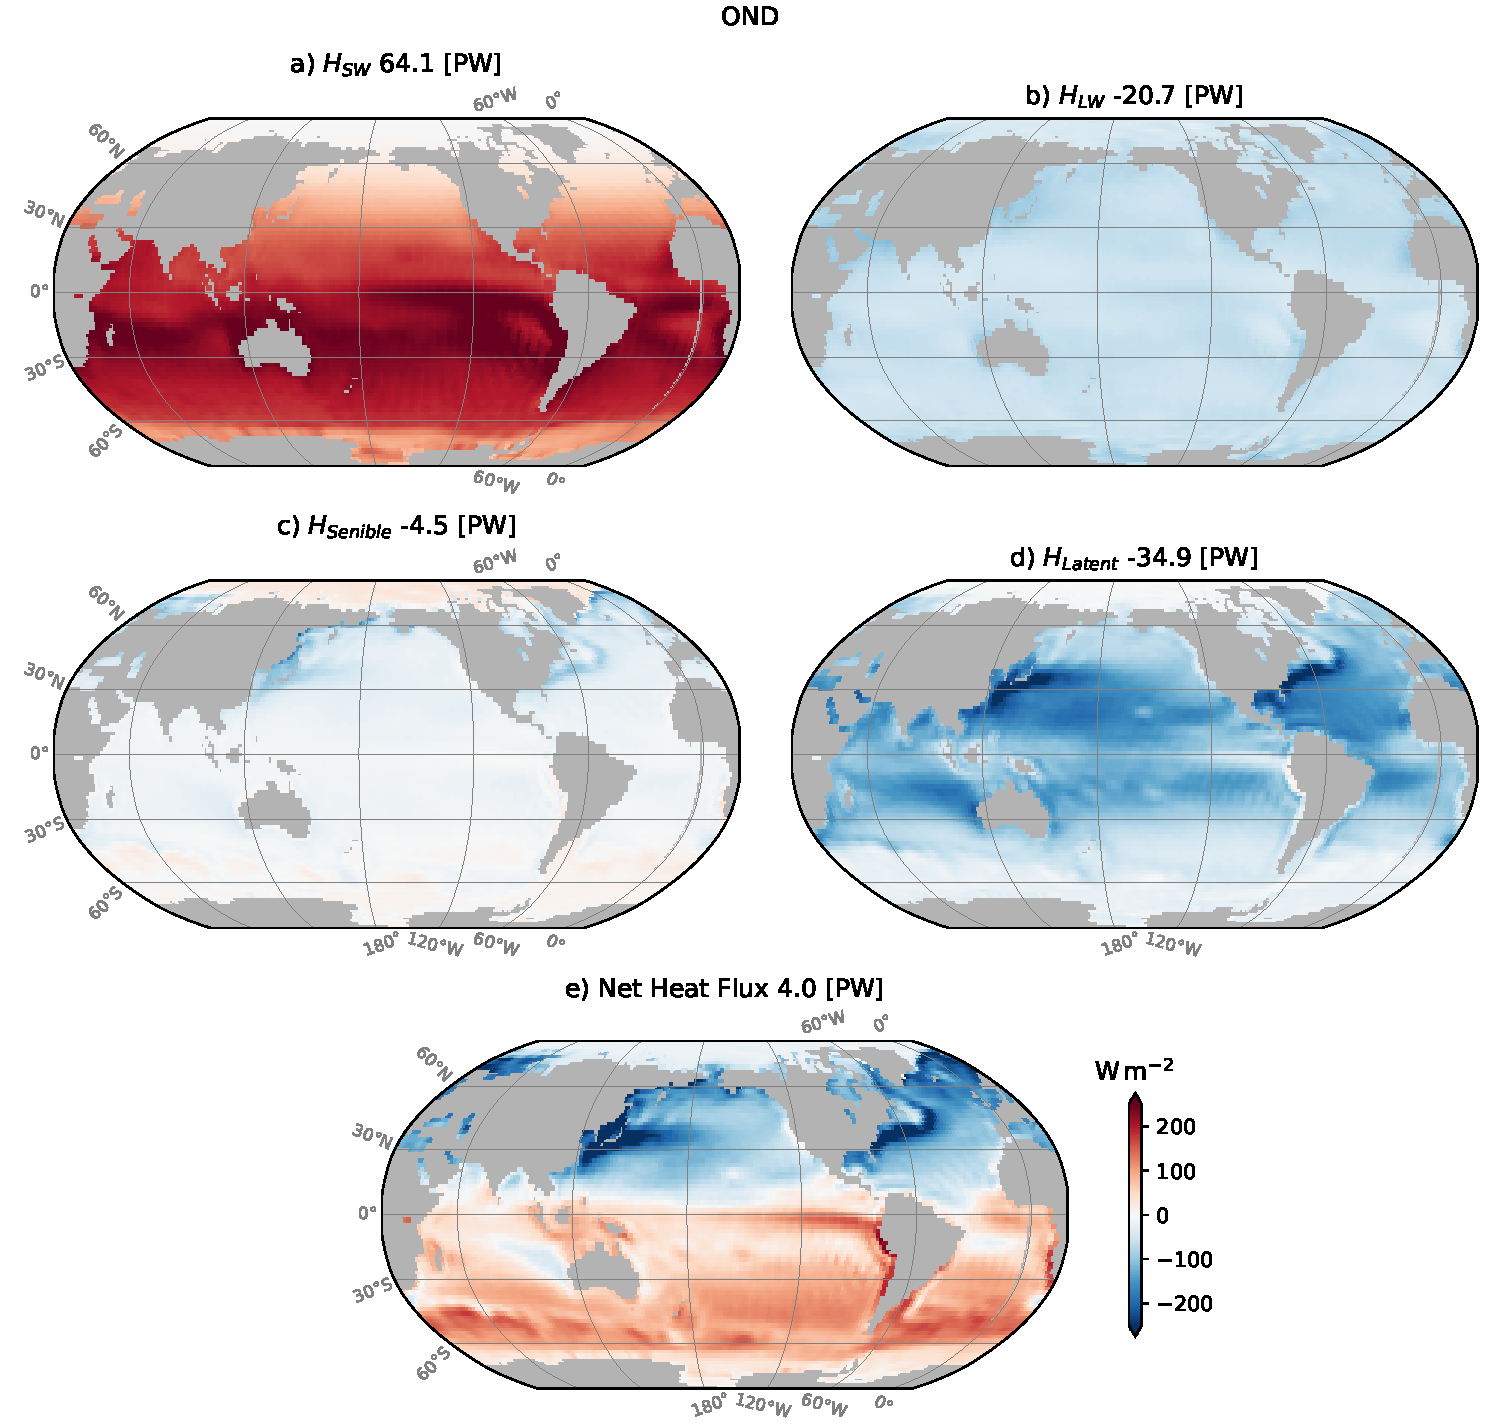
\includegraphics[width=4.5in]{FluxesFigs/SurfaceHeatFluxesOND}
  \caption{Net surface heat fluxes, October to December.  a) Net shortwave heat flux, b) net longwave flux, c) sensible heat flux, d) latent heat flux and e) net heat flux. 
  Data source:  \href{https://psl.noaa.gov/data/gridded/data.ncep.reanalysis.derived.surfaceflux.html}{NCEP1 reanalysis.}  }
  \label{fig:SurfaceHeatFluxesOND}
\end{figure}
\clearpage
\subsection{Longwave radiation (back radiation)}

The earth and ocean emit radiation back into the atmosphere due to their temperature due to blackbody radiation.  If there were no atmosphere, then $H_{LW}$ would depend on temperature of the water to the fourth power, the Stefan-Boltzman constant, and the emissivity of the water.  If this were the case, the ocean would have very large spatial differences in $H_{LW}$ that depended the sea surface temperature.  That is not the case (\fref{fig:SurfaceHeatFluxes}b) because the atmosphere acts as a strong insulator, and back-reflects much of the emission.  Hence, the \emph{net} longwave radiation is surprisingly uniform.  This is tru spatially, as well as temporally  (\fref{fig:SurfaceHeatFluxesJFM}b, \fref{fig:SurfaceHeatFluxesAMJ}b, \fref{fig:SurfaceHeatFluxesJAS}b, \fref{fig:SurfaceHeatFluxesOND}b).  It is indeed surprising that the net back radiation is strongest in the winter when the sea surface is usually colder.

This again points to the difficulty in estimating this flux.  As with shortwave radiation it requires radiometers to measure directly, and some correlation with atmospheric forcing must be made to come up with a net value.

\subsection{Sensible heat transfer}

\begin{figure}[htb]
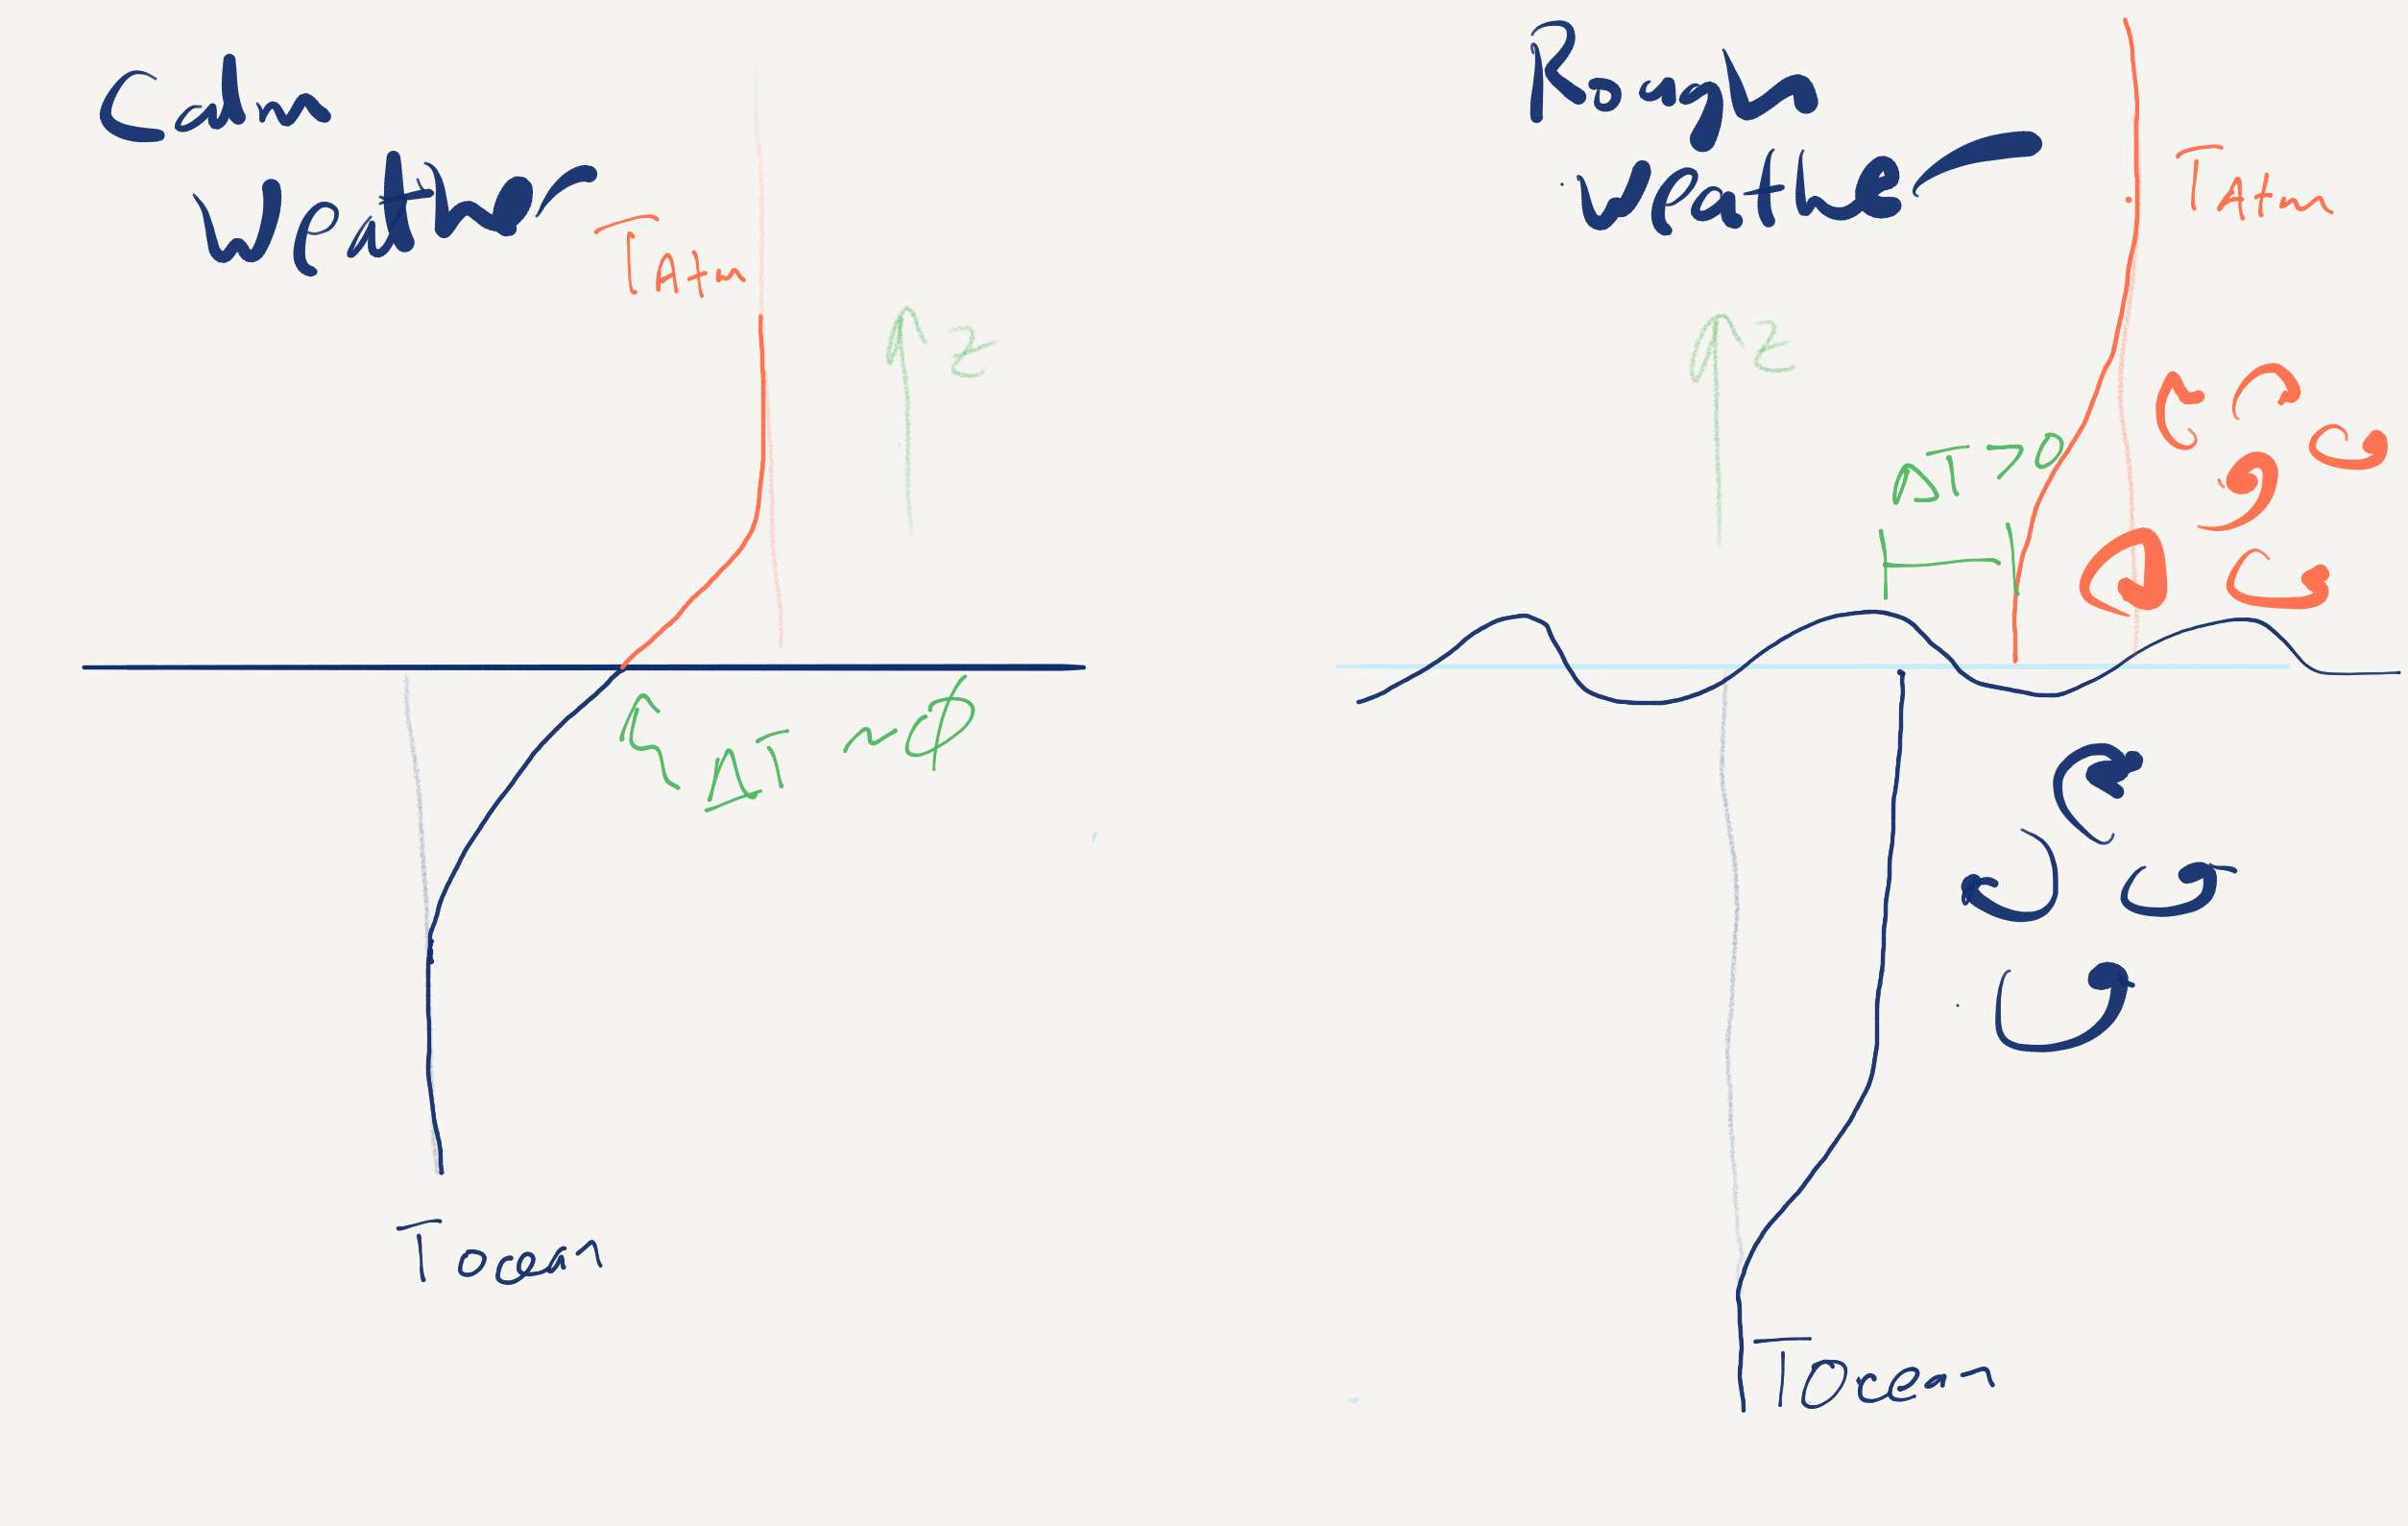
\includegraphics[width=3in]{FluxesFigs/TemperatureProfilesUpperOcean}
 \caption{Sketch of ocean and atmospheric temperature profiles.  During calm weather and stable conditions (warm atmosphere compared to ocean), there is only weak sensible heat transfer.  If there is turbulence in the atmosphere or in the ocean, then the transfer can be greatly enhanced.}
  \label{fig:TemperatureProfilesUpperOcean}
\end{figure}

Sensible heat transfer is the weakest term, despite the fact it is probably what most people think of as how heat is transferred, i.e. when the atmosphere is cold  the ocean loses heat and when it is warm it gains heat.  The heat exchange is usually assumed to be driven by the temperature difference between the top of the ocean and the atmosphere, i.e. $H_{Sensible} \approx k \left(T_{air} - T_{ocean}\right)$ where $k$ is a transfer co-efficient ($W\, K^{-1}$).  However, the temperature of the upper ocean and lower atmosphere of course depends on the flux. So if there is only weak mixing of heat by upper ocean turbulence, the temperature profiles will rapidly equilibrate in thin layers at the interface (\fref{fig:TemperatureProfilesUpperOcean}a).  Conversely, if there is substantial mixing, the temperature difference between the two layers can remain large because heat is mixed away from the interface.  

\begin{figure}[htb]
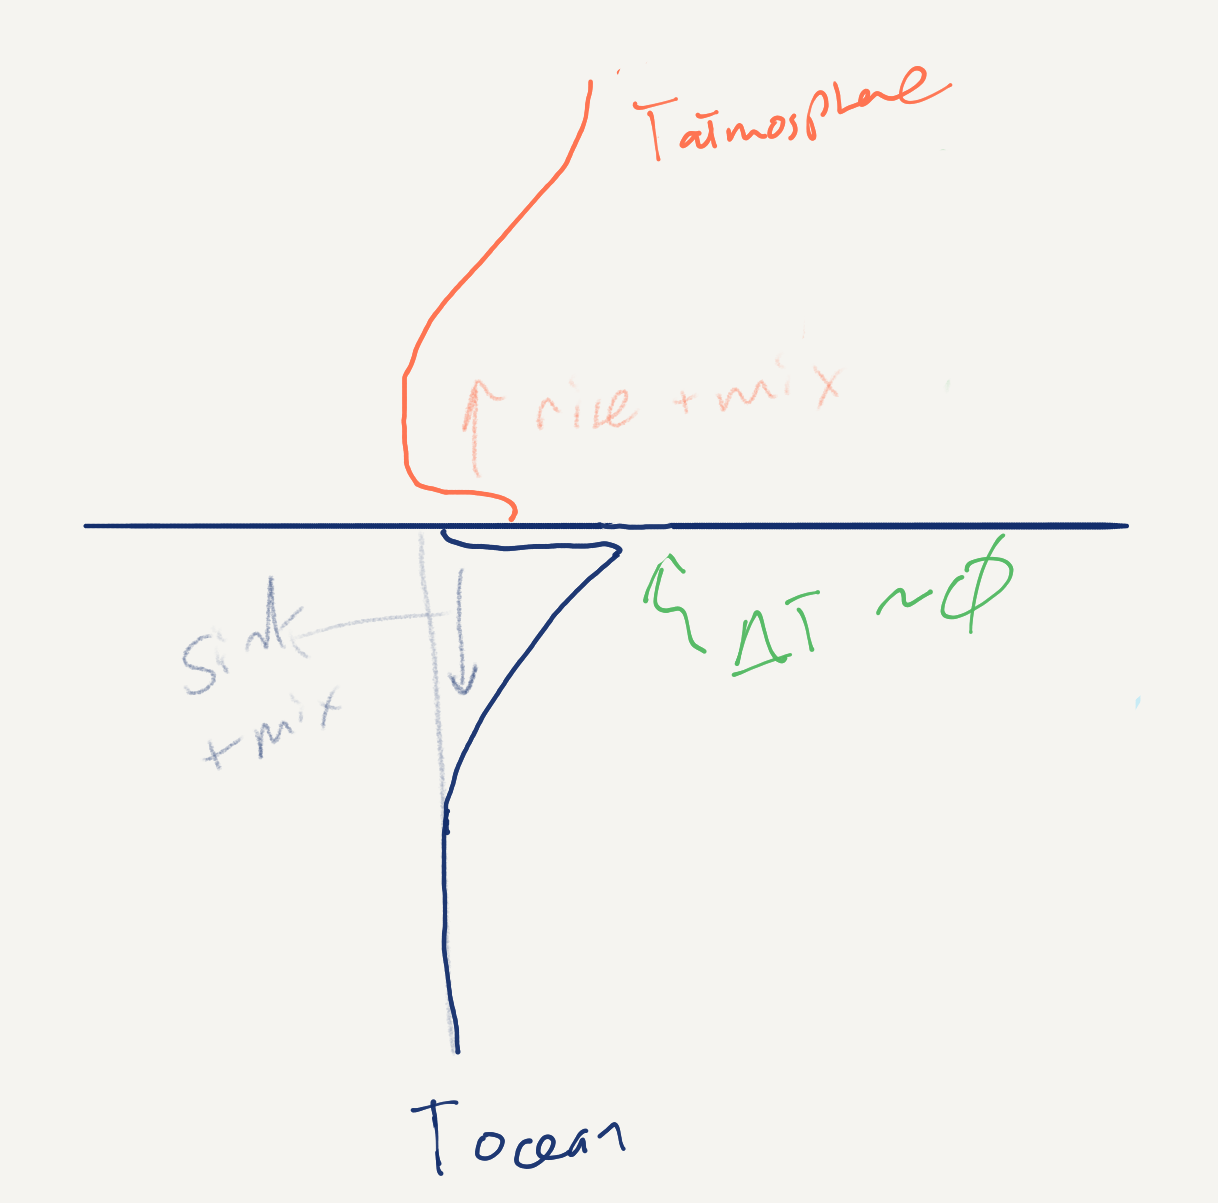
\includegraphics[width=2in]{FluxesFigs/TemperatureProfilesConvect}
 \caption{Sketch of ocean and atmospheric temperature profiles.  During calm weather and stable conditions (warm atmosphere compared to ocean), there is only weak sensible heat transfer.  If there is turbulence in the atmosphere or in the ocean, then the transfer can be greatly enhanced.}
  \label{fig:TemperatureProfilesConvect}
\end{figure}

If the interfaces are unstable, then the ocean (and atmosphere) will tend to ``convect''.  i.e. if the atmosphere at sea level is colder than the ocean, then the cooling of the ocean will lead to cold water on top of warm water and that water will sink.  As it does so, it mixes with the warm water below, and the mixed layer will tend to deepen. Again, mechanical mixing by the wind can enhance this process.

Needless to say, parameterizing these effects to come up with maps like \fref{fig:SurfaceHeatFluxes}c, has required many years of effort and specialized instrumentation \fref{fig:fluxplatforms}.  Measured heat fluxes, as we will see below, are notoriously hard to collect, as are the forcing parameters for those heat fluxes, involving wind speed, ocean current speed, and parameterization for the strength of turbulence in the lower atmosphere and ocean.  For an overview of the state of the art, and the pressing need to improve these measurements see \citet{croninetal19}.  

\begin{figure}[htb]
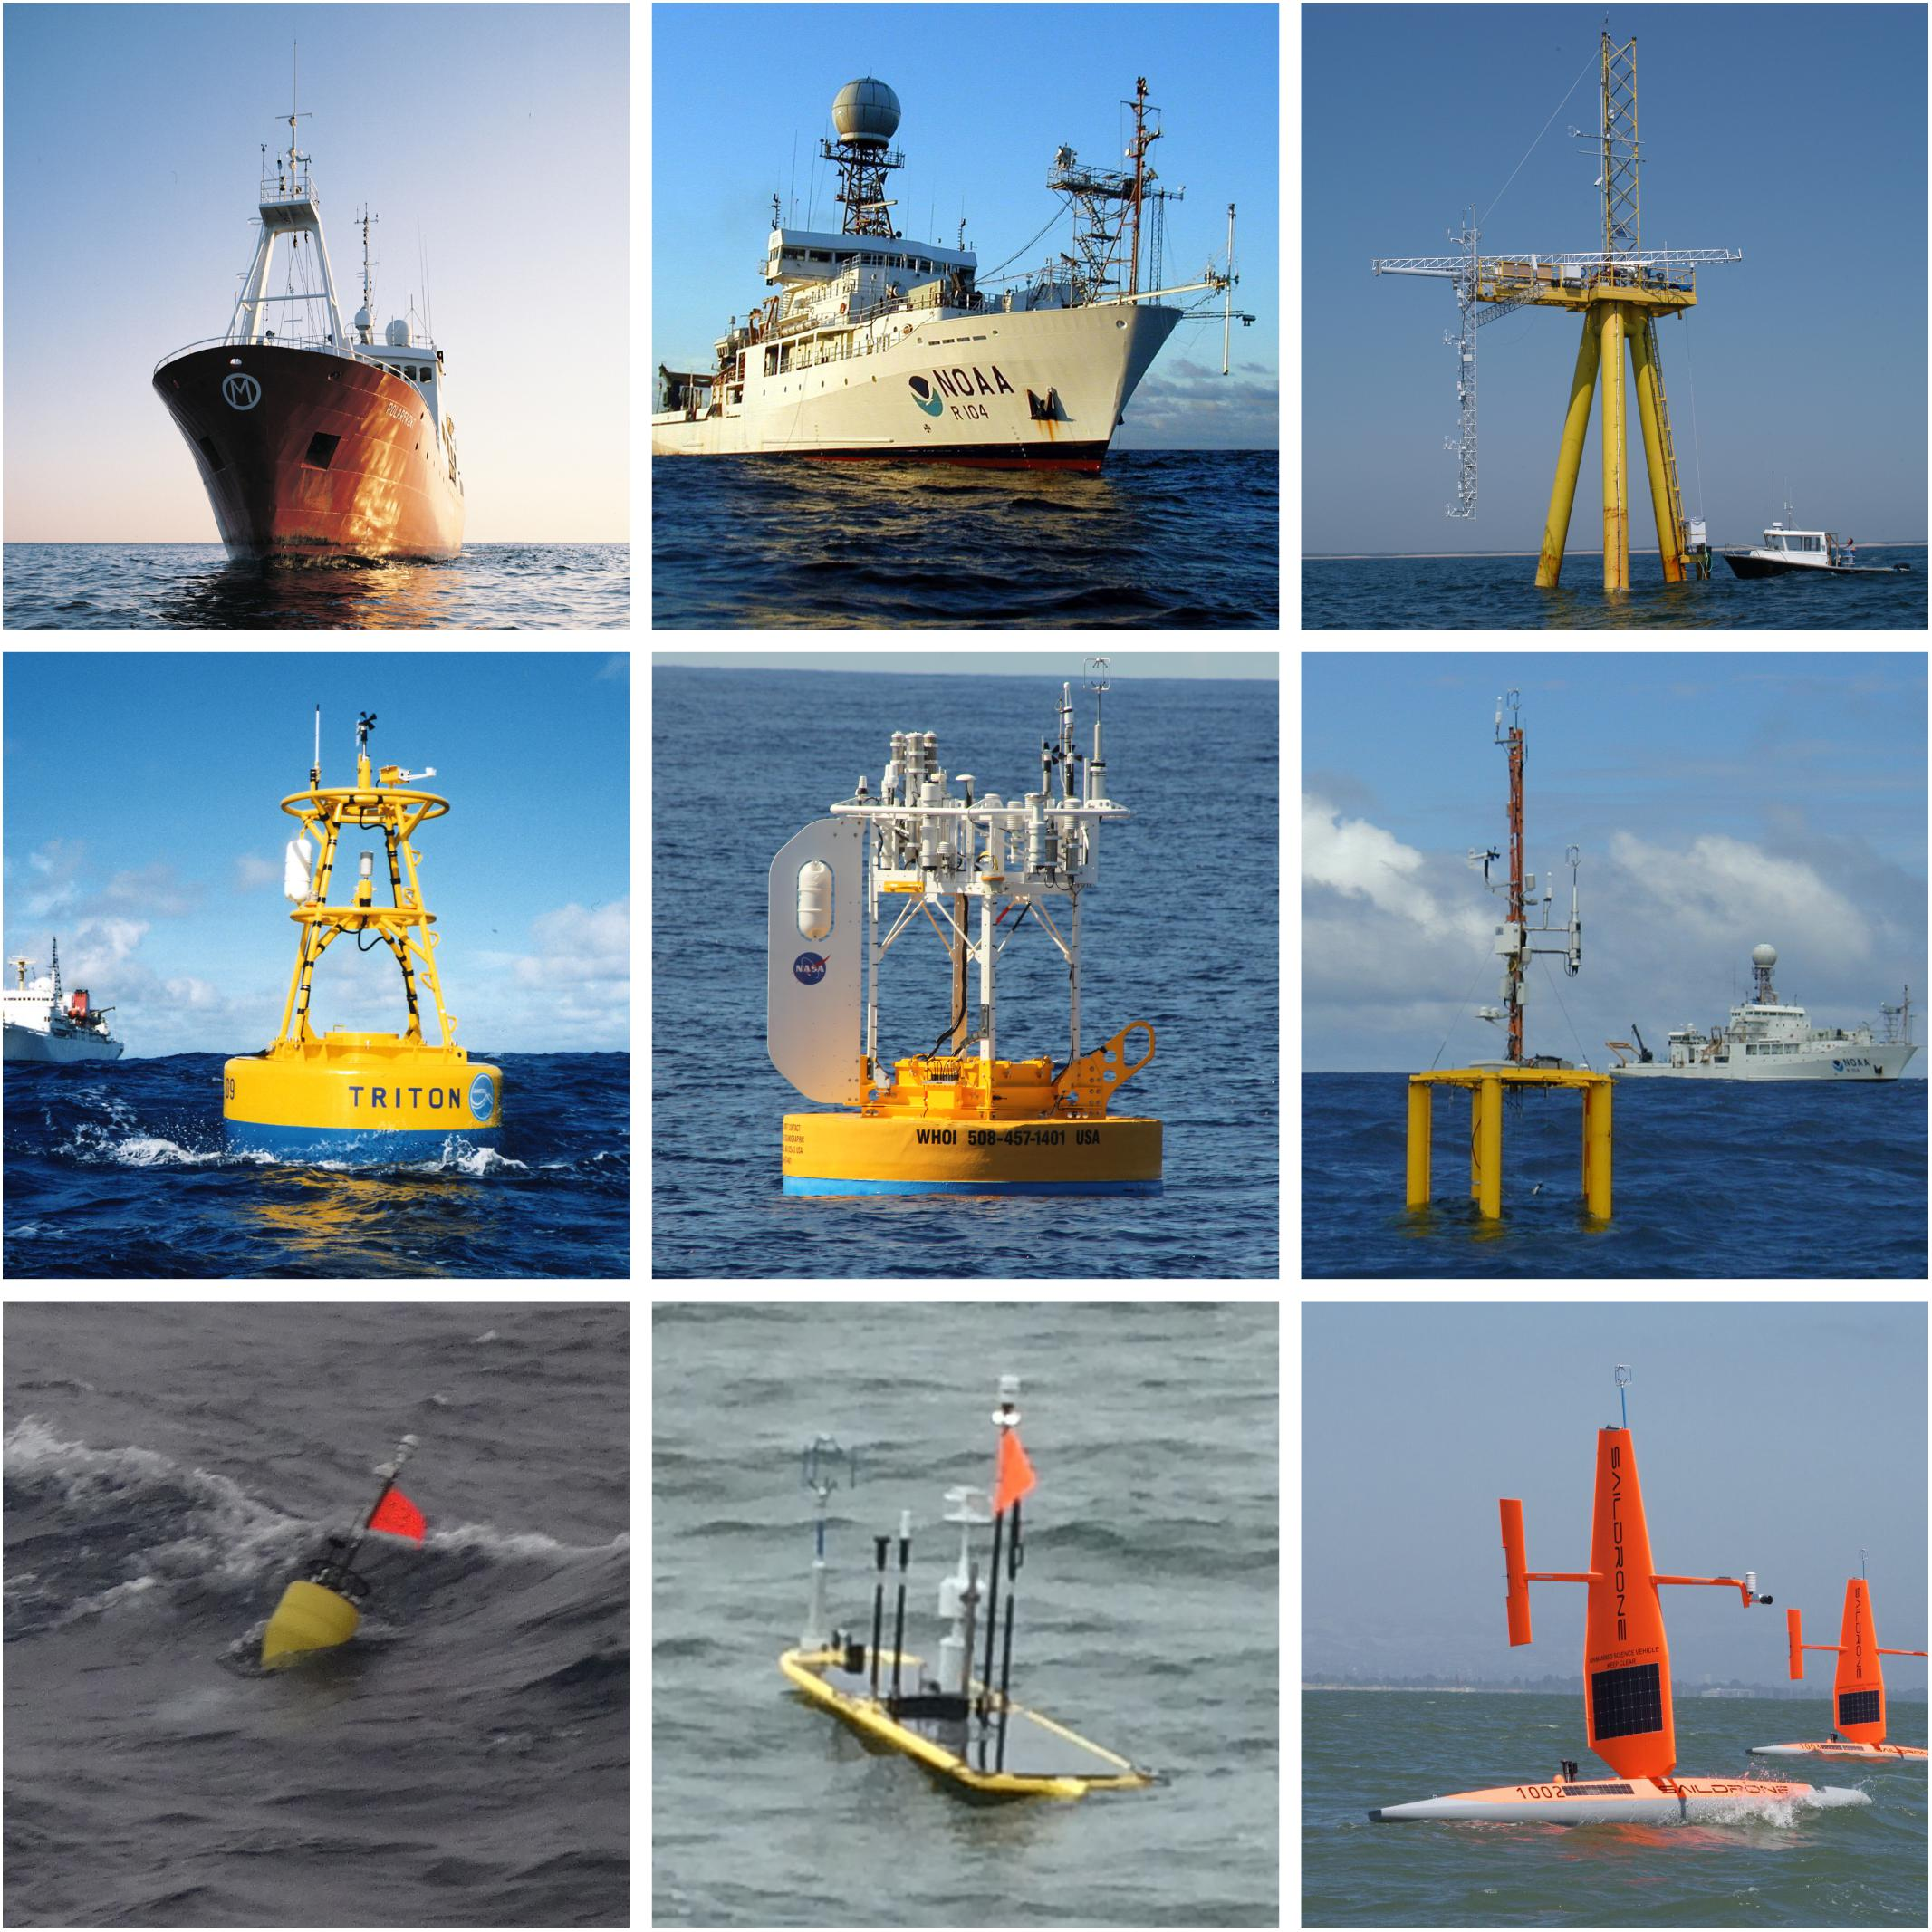
\includegraphics[width=4in]{FluxesFigs/fluxplatforms}
 \caption{Platforms used to measure heat fluxes in the ocean, from \citet{croninetal19}.}
  \label{fig:fluxplatforms}
\end{figure}

The sensible heat losses show a relatively straight forward patterns with the seasons, with a bit of warming of the ocean in the summer, and substantial cooling in the winter (\fref{fig:SurfaceHeatFluxesJFM}c to \fref{fig:SurfaceHeatFluxesOND}c) .  Particularly for the winters there is substantial east-west asymmetry in the ocean's basins, for instance in \fref{fig:SurfaceHeatFluxesJFM}c, there is strong losses off Japan and the Eastern US, centered at around 40 N.  This is due to dry cold winds off the continents, blowing from west to east with the Jet Stream coming into contact with warm water being advected north by the Kuroshio and Gulf Stream.  

\subsection{Latent heat losses}

Latent heat losses are those due to heat used to evaporate water.  Evaporation occurs when the atmospheric humidity, $q$, is less than 100\%.  During evaporation water mass is transferred from the ocean to the atmosphere, \emph{and} the heat stored in that water is transferred from the ocean to the atmosphere.   This transfer is not 100\% efficient because some energy is used to achieve the evaporation, but it does result in a substantial transfer of heat.  

The strength of this transfer depends on the humidity of the ocean directly at the air-sea interface, and hence, just like for the sensible heat transfer, it depends on the turbulence in the atmospheric ``boundary layer'' - if the layer is turbulent because there are strong winds and/or convection, then the moist near-interface air is mixed more thoroughly and the evaporation and exchange of heat is enhanced.   Note that indirectly the exchange depends on the temperature difference between the ocean and the air as cool air can hold more moisture and warm water is more readily evaporated.  

Again, this leads to seasonal changes in the heat flux that mean more evaporative heat flux occurs in the winter than the summer, (\fref{fig:SurfaceHeatFluxesJFM}d to \fref{fig:SurfaceHeatFluxesOND}d).  Further there are clear east-west asymmetries across the basins with the western boundaries at mid-latitude being conspicuous for their evaporative heat loss.  This is because cold dry continental air blows west-east across the warm western boundary currents at these latitudes, leading to substantial evaporation.  

\subsection{Integrated Surface Heat Fluxes}

The maps in \fref{fig:SurfaceHeatFluxes} to \fref{fig:SurfaceHeatFluxesOND} can be integrated to get the net heat flux over the year (\fref{fig:IntegratedHeatFlux}).  Remember that there is a geometric effect of the area of the earth per degree of latitude at the pole goes to zero, where as it is very large at the equator.  Keeping this in mind, the integral around the globe for each degree shows that there is a net heat input at the equator, and losses to the north and south.  Interestingly, in the southern hemisphere, there is a net heat \emph{input} into the ocean between the subpolar band of 40 and 60 S.   The general lack of land mass at these latitudes means that the air has largely equilibrated with the ocean in terms of both temperature and humidity and hence the sensible and latent heat fluxes are negligible.  Note the same thing happens in the North Pacific but is masked in the net by the north Atlantic and the fluxes in the Kuroshio (\fref{fig:SurfaceHeatFluxes}e)

\begin{figure}[htb]
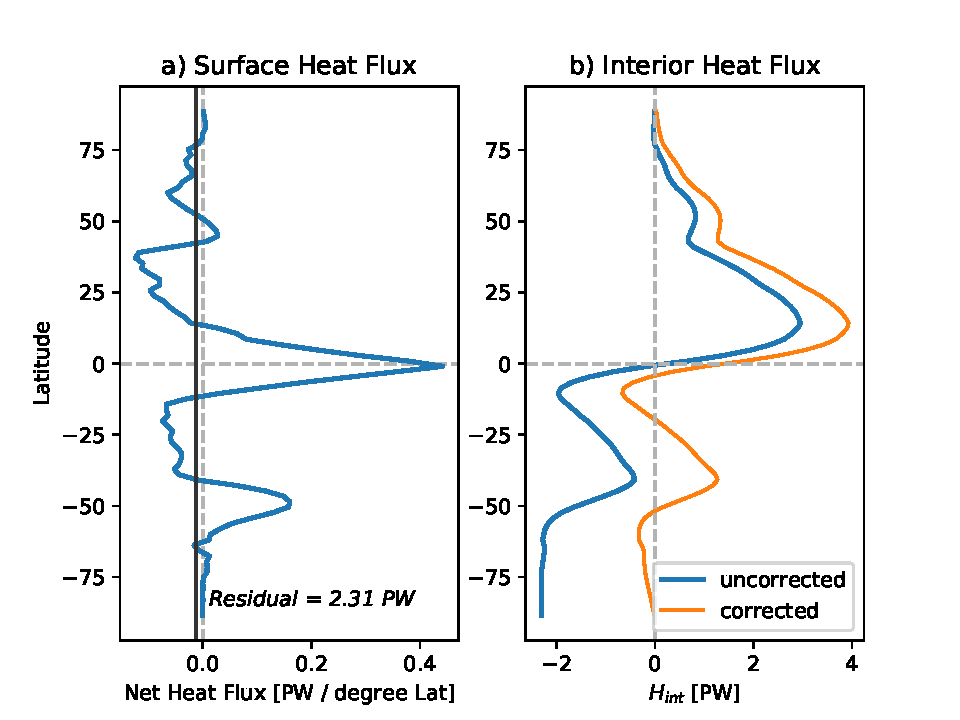
\includegraphics[width=4in]{FluxesFigs/IntegratedHeatFlux}
 \caption{a) Globally integrated annual-mean surface heat flux per one degree of latitude.  The sum of the heat flux is shown as the ``residual'', and is about 4\% of the net incoming radiation. b) the inferred heat transport carried by the ocean, computed by integrating the curve in (a).  Negative heatflux means heat is flowing from north to south.  Theoretically, this should come to zero, so this curve requires correction (orange curve is a crude correction).}
  \label{fig:IntegratedHeatFlux}
\end{figure}

As noted above, the 2.3 PW of residual heating is likely a result of error in the estimate rather than a robust idea of how fast the ocean is heating.  2.3 PW is 4\% of the total incoming flux, and the estimates likely have more than 4\% error in total, so the net flux is not significantly different from zero.  

On moderate time scales it is often helpful to think of the ocean as being in steady-state, so in this case it is helpful to think of the ocean as not changing temperature.  On the other hand, if there is a net flux of heat into the ocean at some latitude, and a net flux out at another latitude, either the ocean where there is a net heatflux in is getting warmer and warmer, or it is transporting heat to the region where it loses heat, as sketched in \fref{fig:HeatFluxBoxes}. 


\begin{marginfigure}
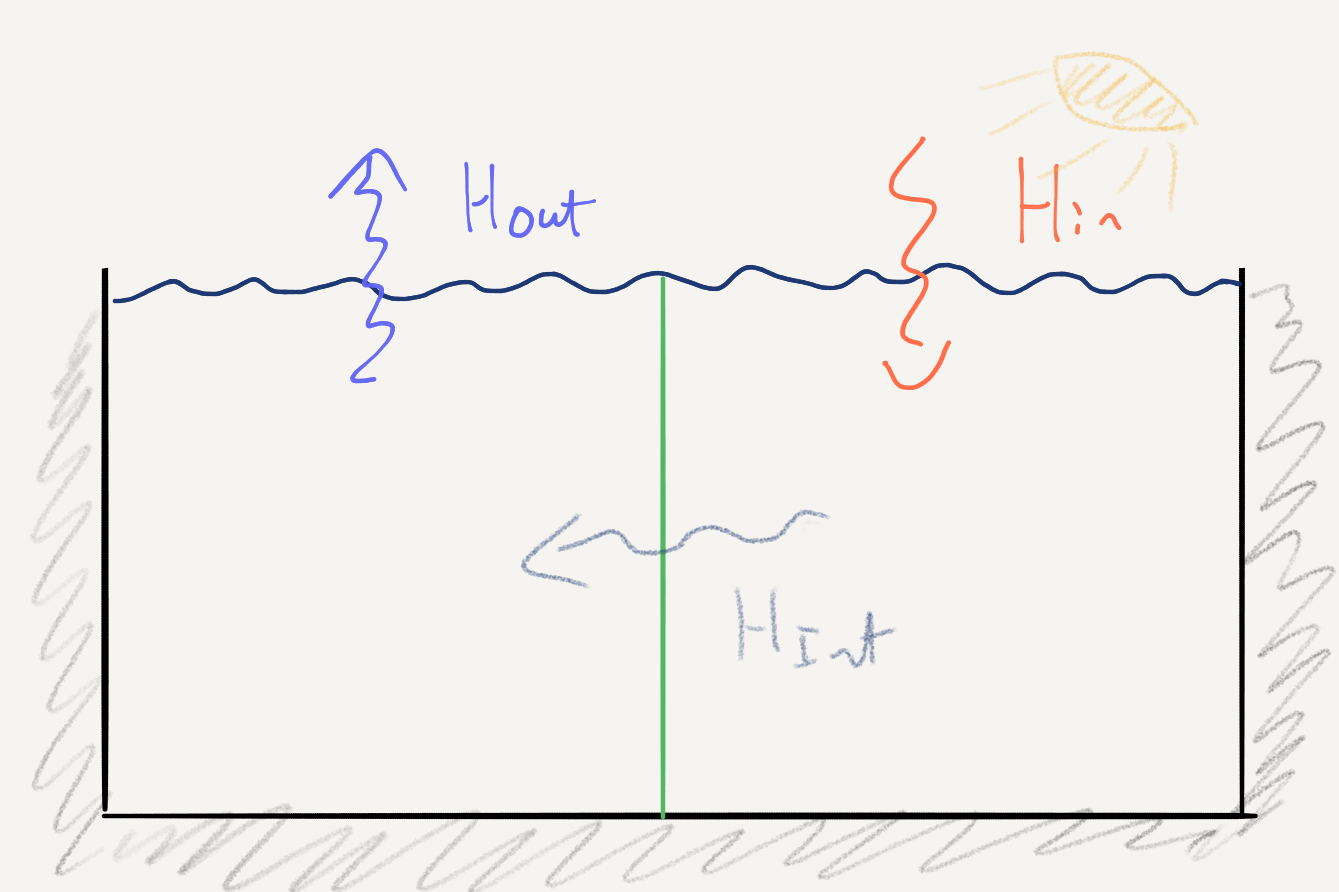
\includegraphics[width=2in]{FluxesFigs/HeatFluxBoxes}
 \caption{Schematic two-box representation where the right-hand box is being heated, the left-hand box cooled, and a heat flux in the interior of the box is assumed to be from warm to cold.}
  \label{fig:HeatFluxBoxes}
\end{marginfigure}

Extending this idea to many boxes is straight forward, but we have to remember that the boxes have a heat source both at the surface, and an interior flux on both sides of the box.   (\fref{fig:HeatFluxSchematic}). If we assume steady state and that these heat fluxes balance, then we have $H_{in}^{(N)} = H_{in}^{(N-1)} + H_S^{(N)}$ where the bracketed superscripts refer to the cell number. Surface fluxes are defined as positive into the ocean, and interior fluxes are defined as positive if they are to the north.  We can also write this as $\Delta H_{in}^{(N)} = H_S^{(N)}$ and we can see that if we have a positive heat flux into the ocean, then the northward heat flux must grow.  Because this relation starts at a pole, where the interior heat flux is zero, the interior heatflux at any given latitude is the sum of the surface fluxes to the south of that latitude: 
\begin{equation}
    H_{in}^{(N)} = \sum_{i=0}^N H_{S}^{(i)}
\end{equation}
This gives us the curve in \fref{fig:IntegratedHeatFlux}b, which shows northward heatflux in the northern hemisphere and southwards in the southern hemisphere.  Again, there is a residual heat flux, so this procedure does not yield a completely sensible curve with large southwards heatflux at the southernmost ocean cell, so a correction is applied that removes the mean flux.  

\begin{marginfigure}
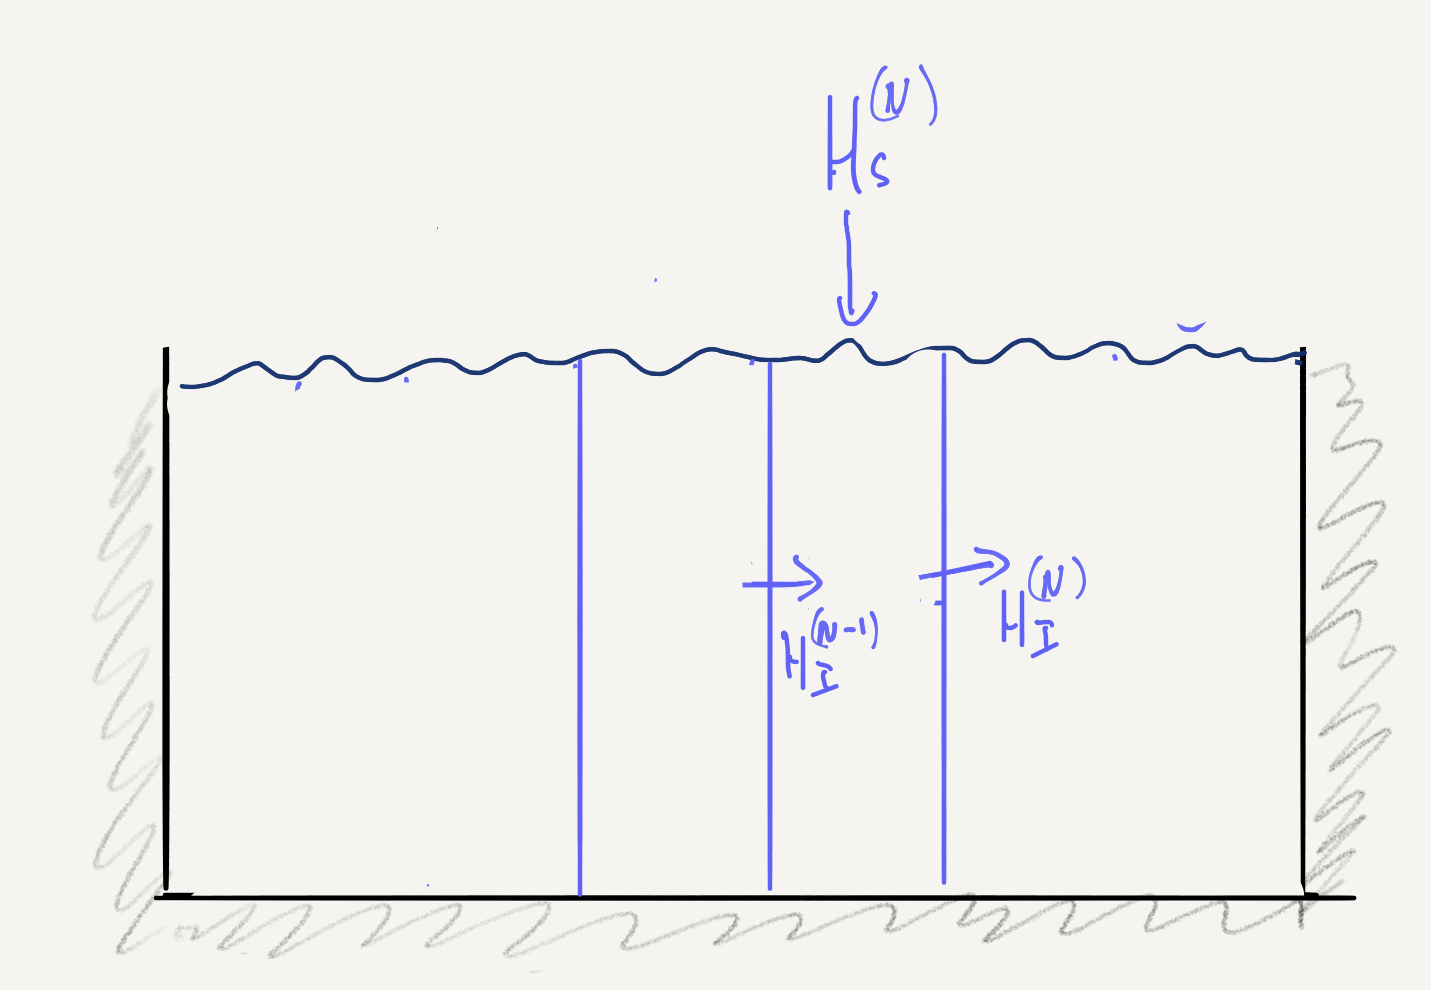
\includegraphics[width=2in]{FluxesFigs/HeatFluxSchematic}
 \caption{Schematic two-box representation where the right-hand box is being heated, the left-hand box cooled, and a heat flux in the interior of the box is assumed to be from warm to cold.}
  \label{fig:HeatFluxSchematic}
\end{marginfigure}

Direct estimates of the interior fluxes have also been made from ocean-based measurements, and a number of these are compared in \fref{fig:GanachaudWunsch03Fig5}.  The level of variability in these estimates indicates the difficulties in making these types of estimates, even if the patterns make the sense.  

\begin{figure}
\begin{center}
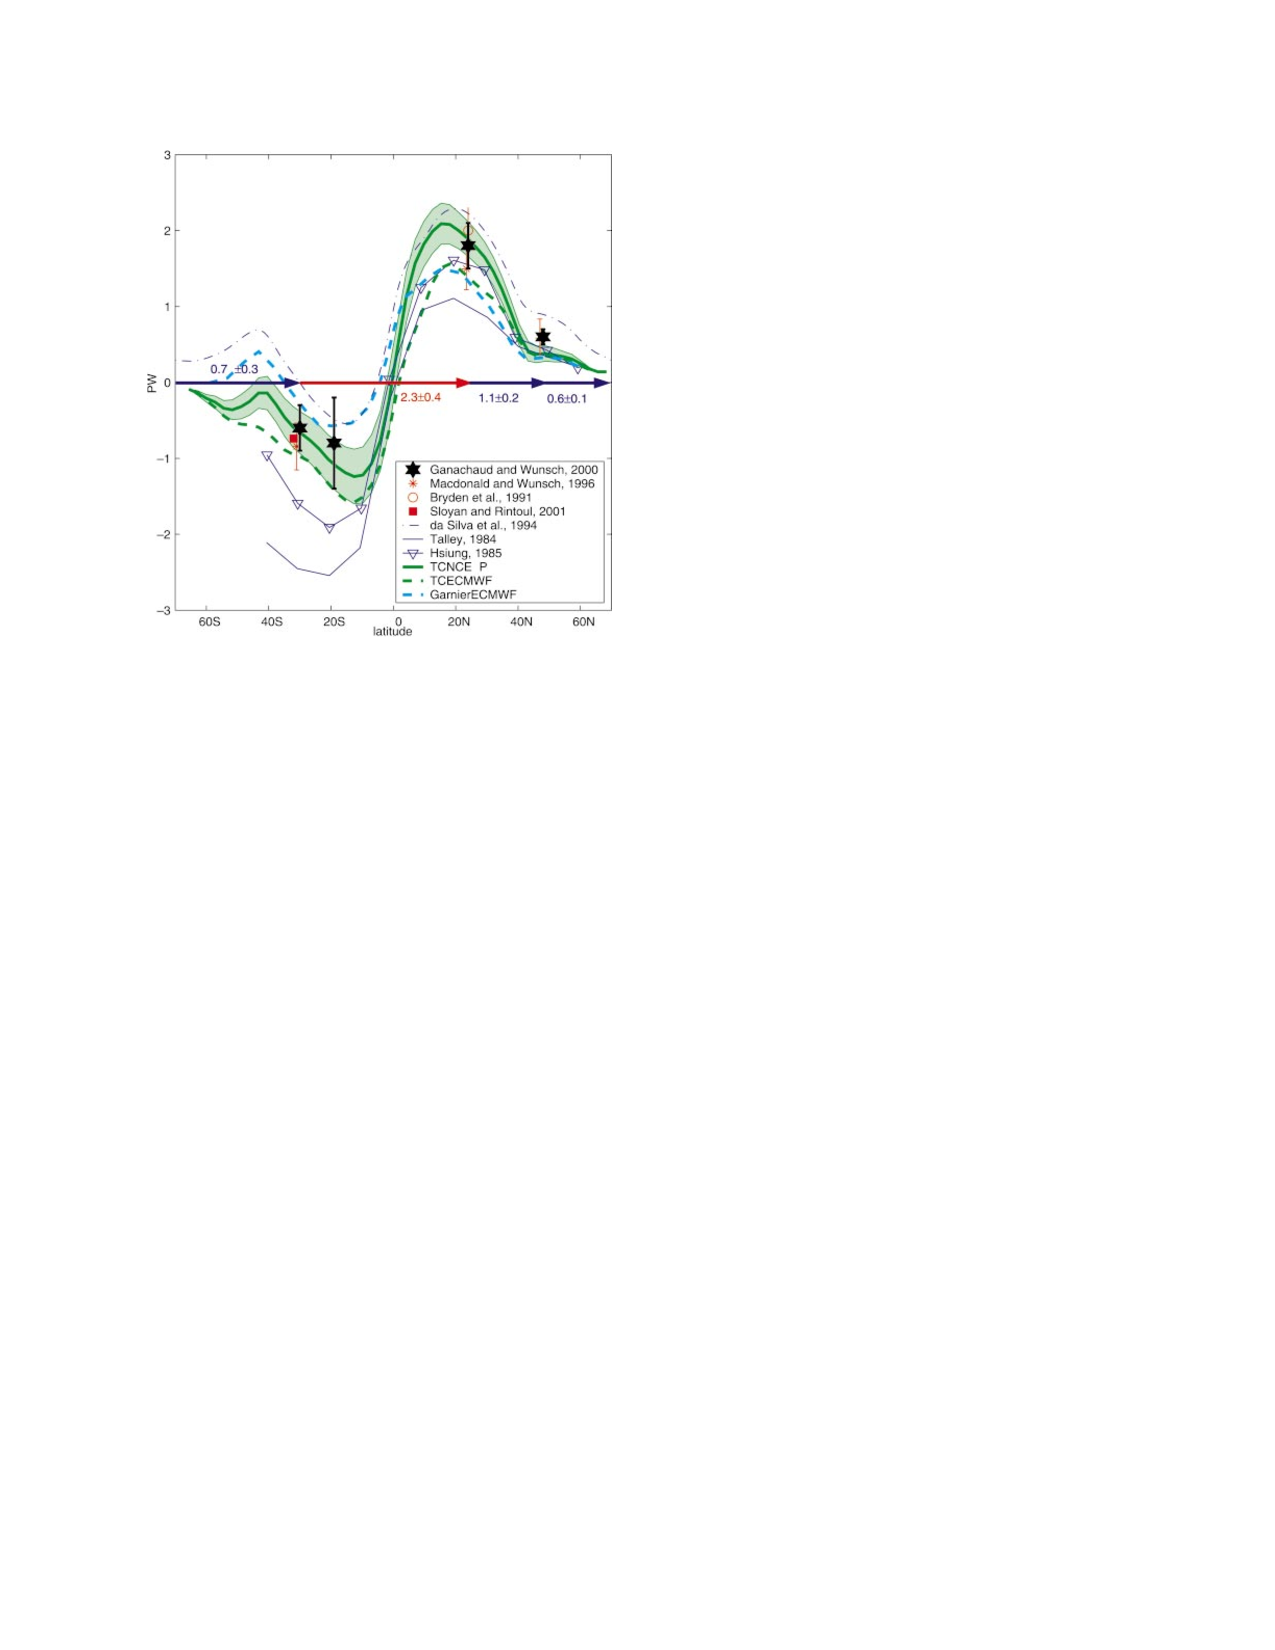
\includegraphics[width=2.7in]{FluxesFigs/GanachaudWunsch03Fig5}
 \caption{Estimates of heat transport by the world's oceans \citep{ganachaudwunsch03}.}
  \label{fig:GanachaudWunsch03Fig5}
\end{center}
\end{figure}

If we look at these fluxes by ocean basin, then there are substantial differences between the Atlantic ocean and the Pacific/Indian Oceans in terms of the structure of the heat flux.  In the Atlantic ocean the heat flux is everywhere north.  This is because the heat flux at the equator is relatively weak, and there is substantial heat flux in the south Atlantic.  


\begin{figure}
\begin{center}
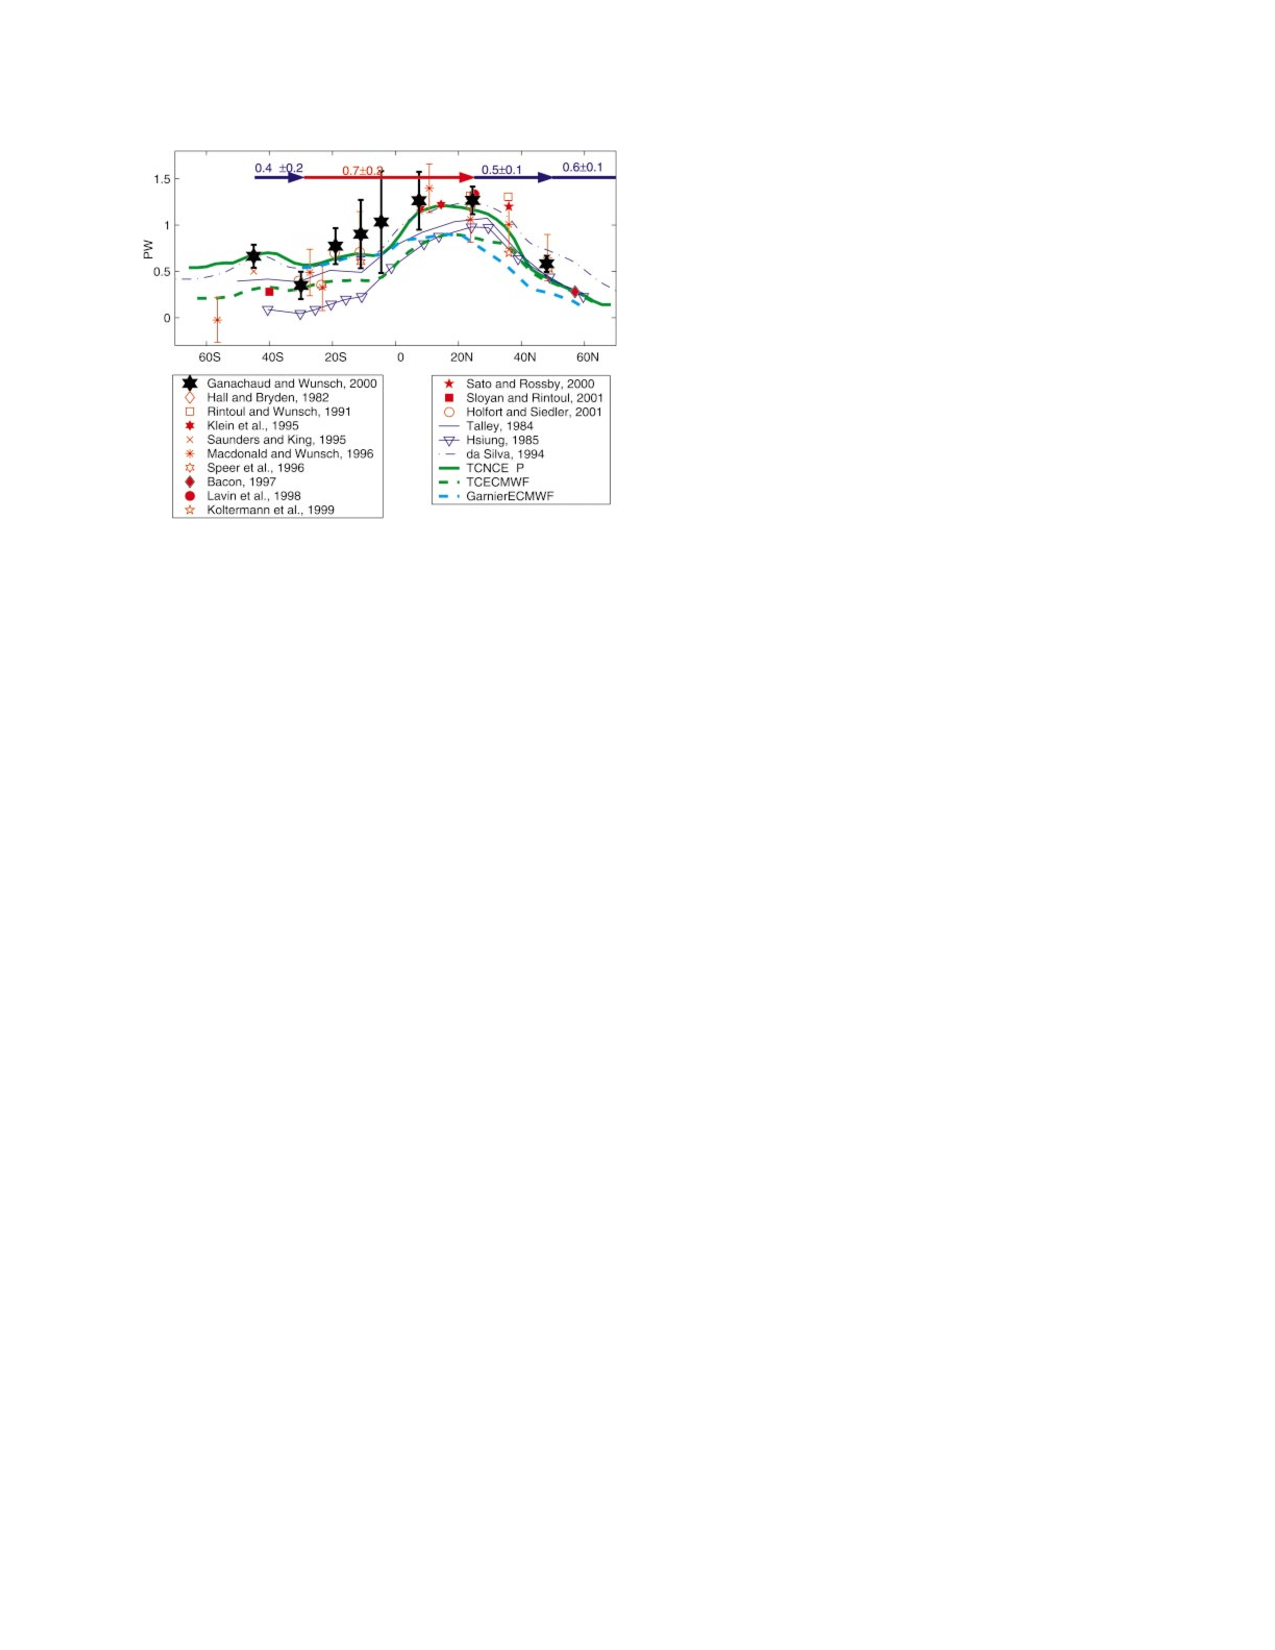
\includegraphics[width=2.7in]{FluxesFigs/GanachaudWunsch03Fig3}
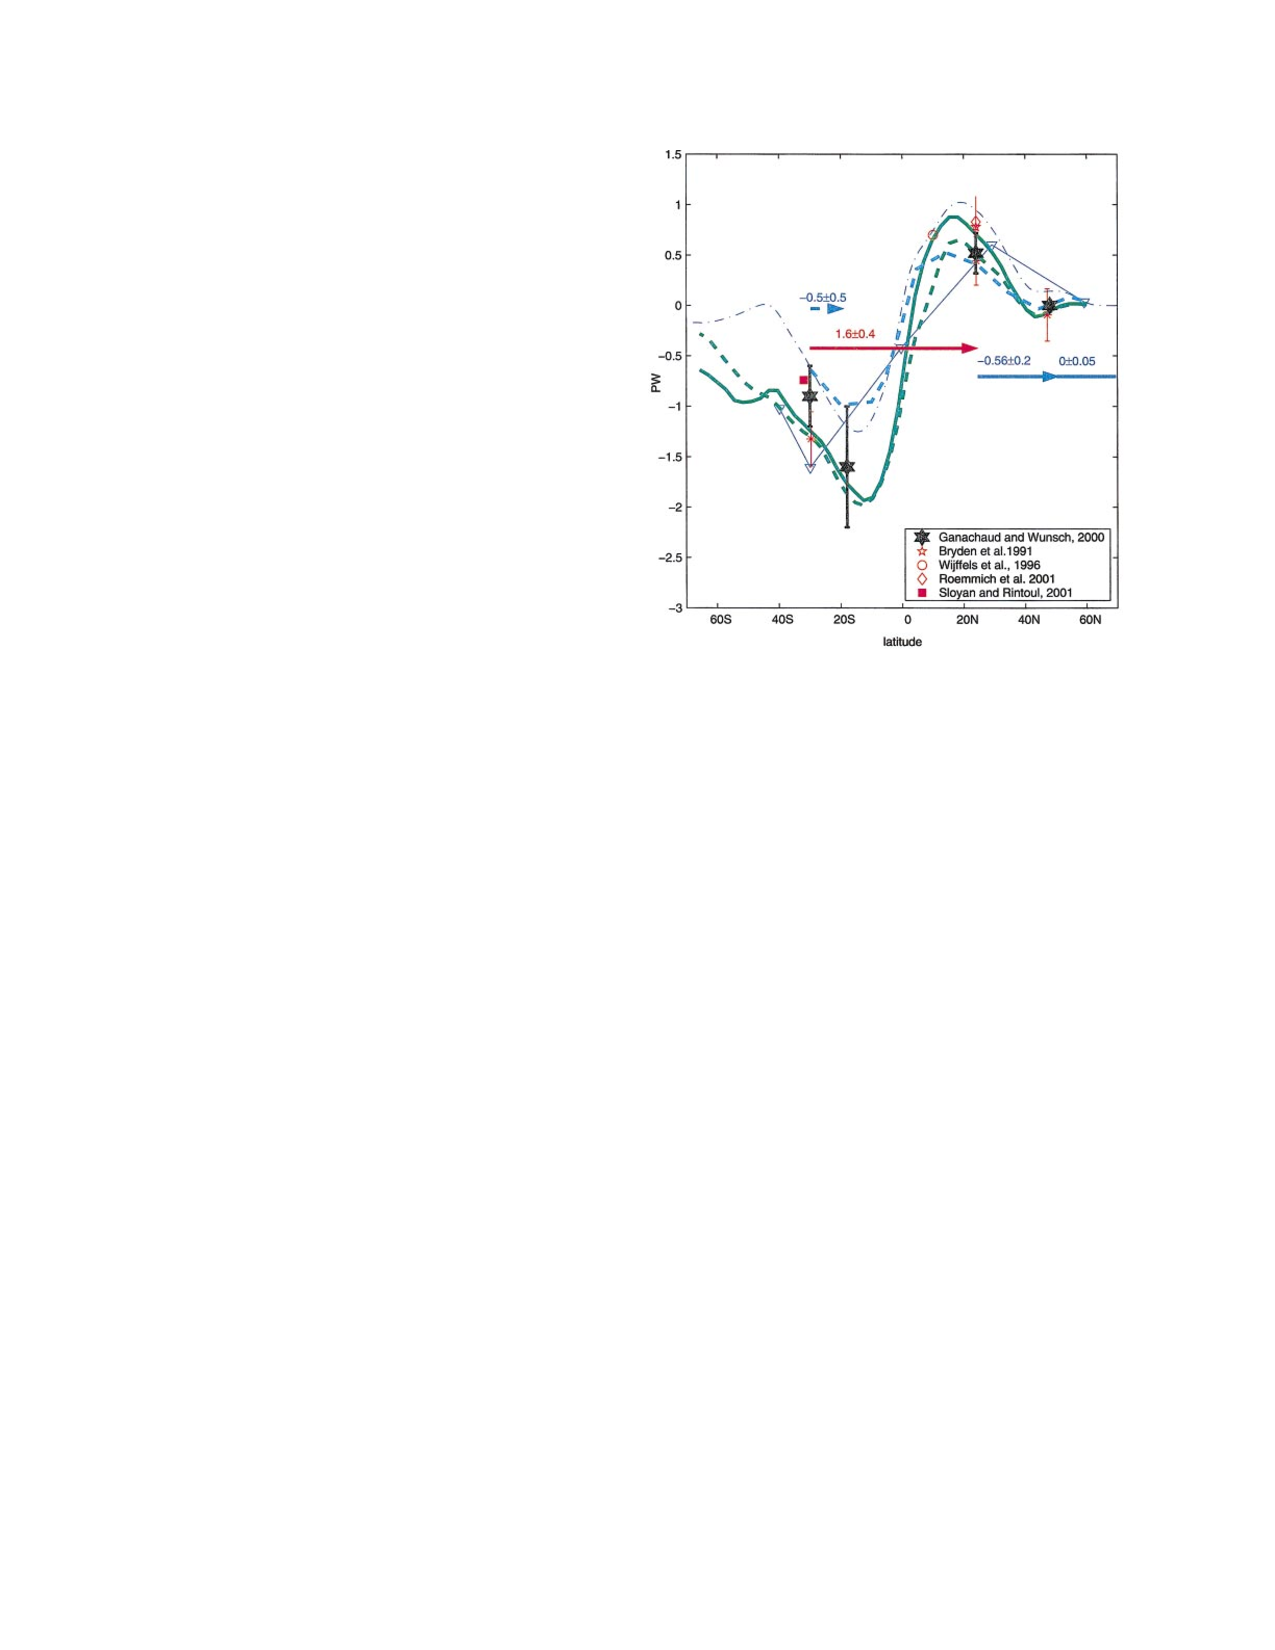
\includegraphics[width=2.7in]{FluxesFigs/GanachaudWunsch03Fig4}
 \caption{Estimates of heat transport in the Atlantic (upper panel) and Pacific and Indian oceans (lower panel)\citep{ganachaudwunsch03}.}
  \label{fig:GanachaudWunsch03Fig3_4}
\end{center}
\end{figure}

We have said nothing about what drives these heat fluxes, however, the basic idea is that warm water is less dense, and hence more buoyant, whereas cold water is less buoyant.  Just like in an estuary, this creates north-south pressure gradients that drive the warm water northwards.  

\marginpar{Make a demo about this!}

\section{Surface freshwater fluxes}

The ocean has a large reservoir of salinity compared to the rate of inputs (from rivers) and outputs (from forming \Wikiref{evaporite}s), to the point that the mass of salt in the ocean can be regarded as a constant on the timescale of decades to centuries.  Given the volume of the ocean is approximately $1.335\times10^{18}\ \mathrm{m^3}$, and a typical density is $1030\ \mathrm{kg\,m^{-3}}$, and salinity is $S\approx35 \ \mathrm{ppt}$, the mass of salt in the oceans is approximately $4.5\times10^{19} \ \mathrm{kg}$.  Conversely, rivers deliver on the order of  $3\times10^{12} \ \mathrm{kg}$ of salt per year, so, in order to increase ocean salinity by one part per thousand, it would take more than 450,000 years of salt input.  Given that much of this input is balanced by output to forming evaporites, we tend to think of the salt balance as not changing over sub-geological timescales.  

Of course this doesn't mean that salinity is constant in the ocean!  Salinity is almost zero in rivers, and is zero in rainfall and at locations where these meet the ocean the salinity drops.  Conversely if there is evaporation and ice formation, then salinity is left behind and the ocean is saltier in those locations.  When we think about the large-scale budgets then, we often think of them as freshwater budgets, with the understanding that these are also salinity budgets.  

\subsection{Evaporation and precipitation patterns}

As noted above, evaporation is complicated to estimate because it depends on the temperature difference of the ocean ant atmosphere, the humidity of the atmosphere, and all of those parameters depend on the turbulence near the boundary between the two fluids. Many of the spatial patterns of evaporation are the same as those for latent heat loss (\fref{fig:E-P}a), with evaporation largest where cold dry air passes over warm ocean currents.


\begin{figure}
\begin{center}
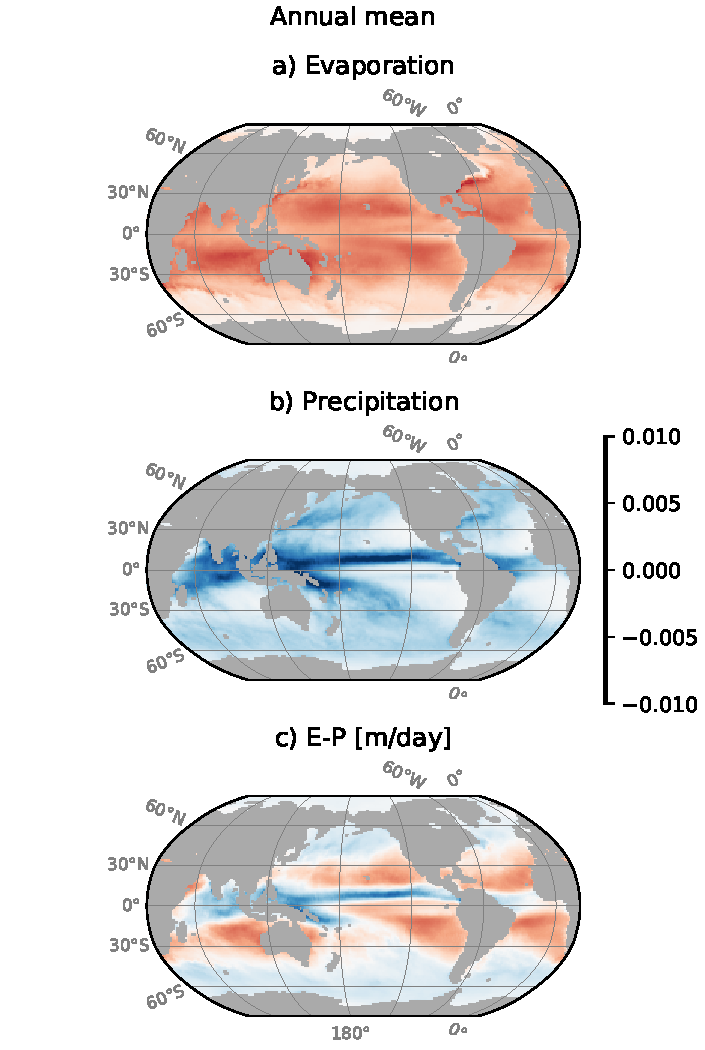
\includegraphics[width=4in]{FluxesFigs/E-P}
 \caption{Annual average evaporation and precipitation (from \href{https://www.ecmwf.int/en/forecasts/datasets/reanalysis-datasets/cera-20c}{ECMWF-CERA-20c} re-analysis).  }
  \label{fig:E-P}
\end{center}
\end{figure}

Freshwater re-enters the ocean via precipitation and rivers.  The precipitation patterns are largely driven by the \Wikiref{Hadley cell} circulation of the atmosphere, with large upward motion at the equator driving strong rainfall there (\fref{fig:E-P}).  The subpolar latitudes see more rainfall as well because there is also rising air in the midlatitude cell, centred at about 60 degrees.  Dry air predominates at the subtropical latitudes where this air tends to be subsiding. 

\begin{marginfigure}
\begin{center}
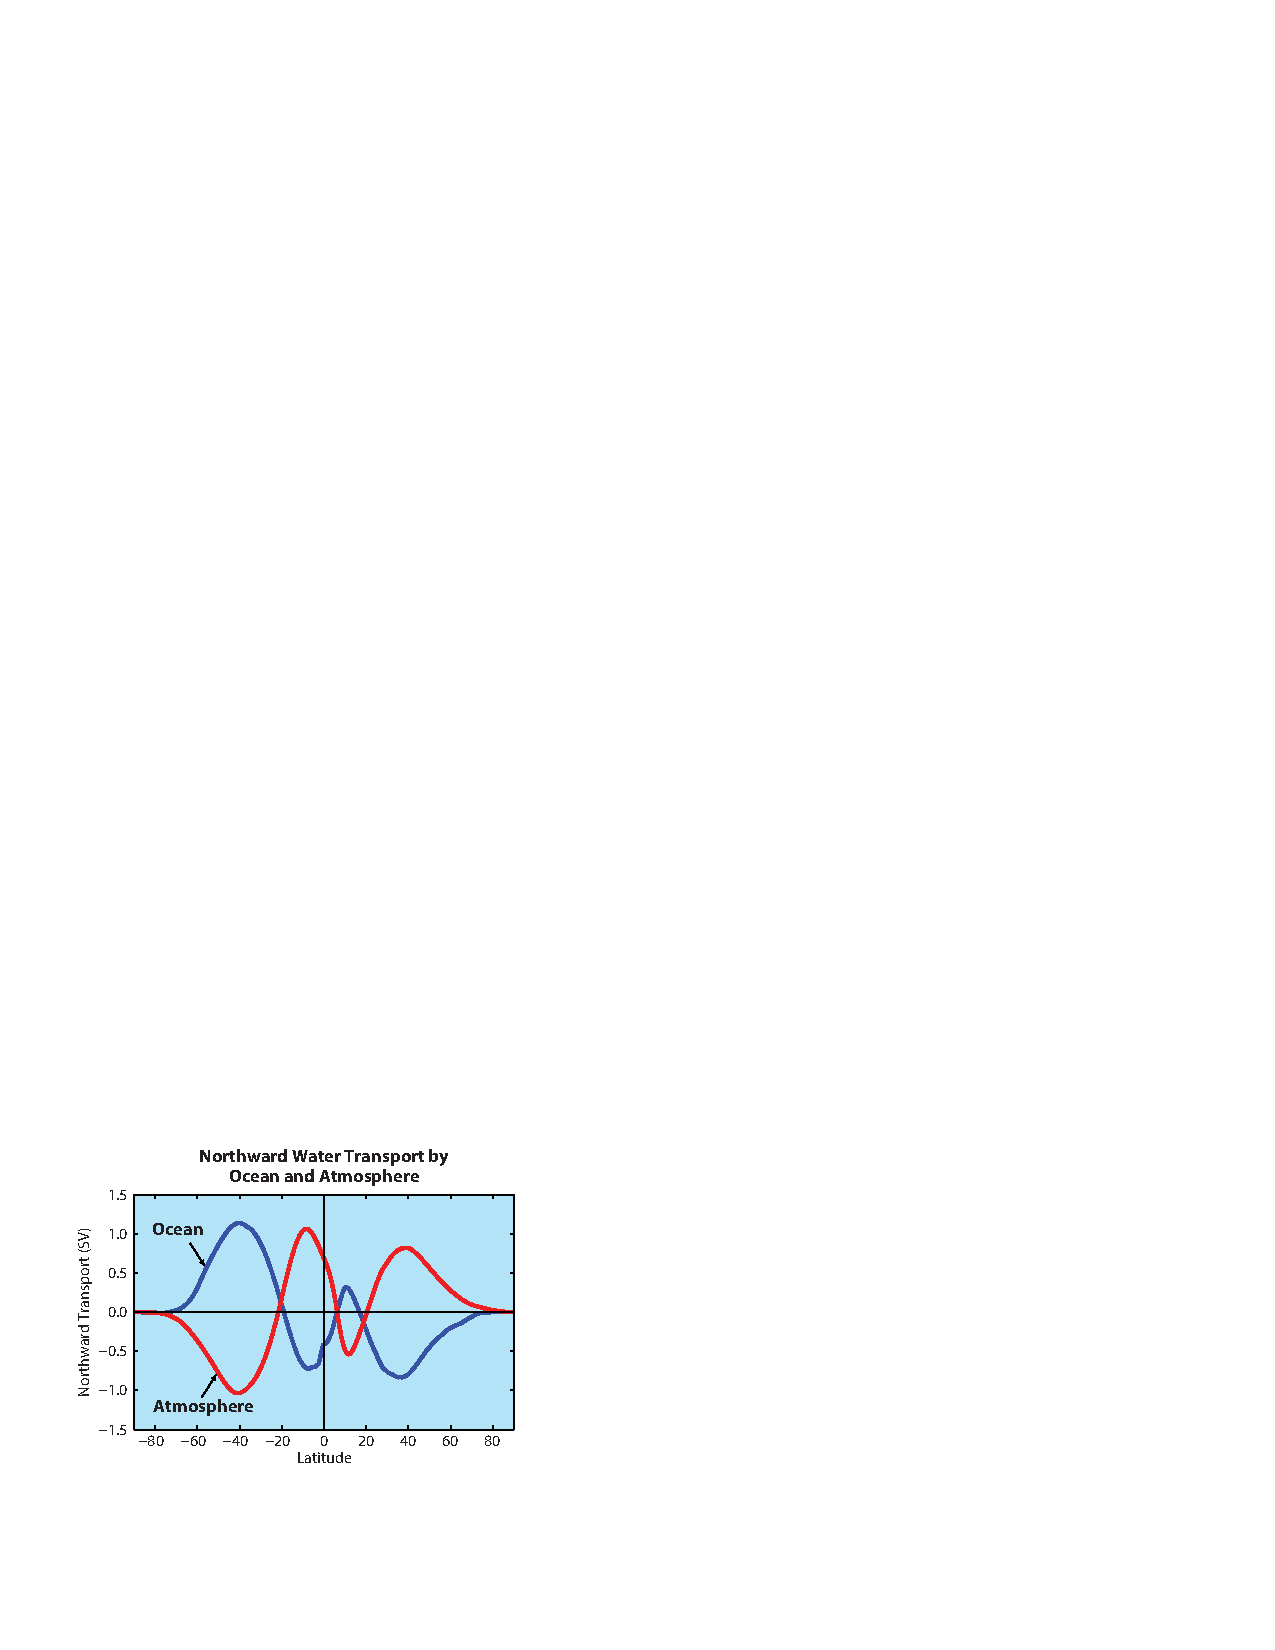
\includegraphics[width=2.5in]{FluxesFigs/Schmitt18Fig5}
 \caption{Net annual fresh-water transport \citep[from][Fig.\ 5]{Schmitt18}.  The ocean curve is estimates by integrating the net surface flux curve integrated from \fref{fig:E-P}, as described above for heat.  The atmospheric curve is estimated from the ERA moisture transport simulations.  }
  \label{fig:Schmitt18Fig5}
\end{center}
\end{marginfigure}

The net pattern of evaporation minus precipitation generally says that moisture is removed from the oceans in a band from approximately 5 degrees to 35 degrees, and in the net, precipitates near the equator and north of 40 degrees.  As with heat, this necessitates a transport of freshwater from places of excess precipitation to places of excess evaporation if the ocean is to stay in approximate steady state (\fref{fig:Schmitt18Fig5}).   


\chapter{Fluxes and transports in the ocean}
\label{ch:fluxestransports}

We saw in the previous chapter that heat and freshwater can enter and leave the ocean at the surface.  We also \emph{inferred} that it must be transported from sources to sinks at the surface if the ocean is believed to be in a quasi-steady state.  We call this an \emph{inverse estimate} because we infer the inner workings of the ocean from its external forcing.  In this chapter we start grappling with \emph{how} that transport takes place, and how we might quantify and measure it.  There are actually \emph{many} processes involved in the transport of heat from the equator poleward, and trying to understand them all is one of  the main challenges of oceanography.  Given that, this chapter only gives some tools to start understanding fluxes and transports, and as such uses some simple examples.  

Note that temperature, (or heat), for instance, can change at a location away from the surface in two possible ways.  Currents can bring water with a different temperature from somewhere else; we call this an \emph{advective flux}.    Conversely the water can exchange heat via mixing, both at the large scale (stirring) and ultimately at the small scale (molecular diffusion).  We call this a \emph{diffusive flux}.  

\section{Advective fluxes and transport}
\subsection{Advective flux} 

\begin{marginfigure}
\begin{center}
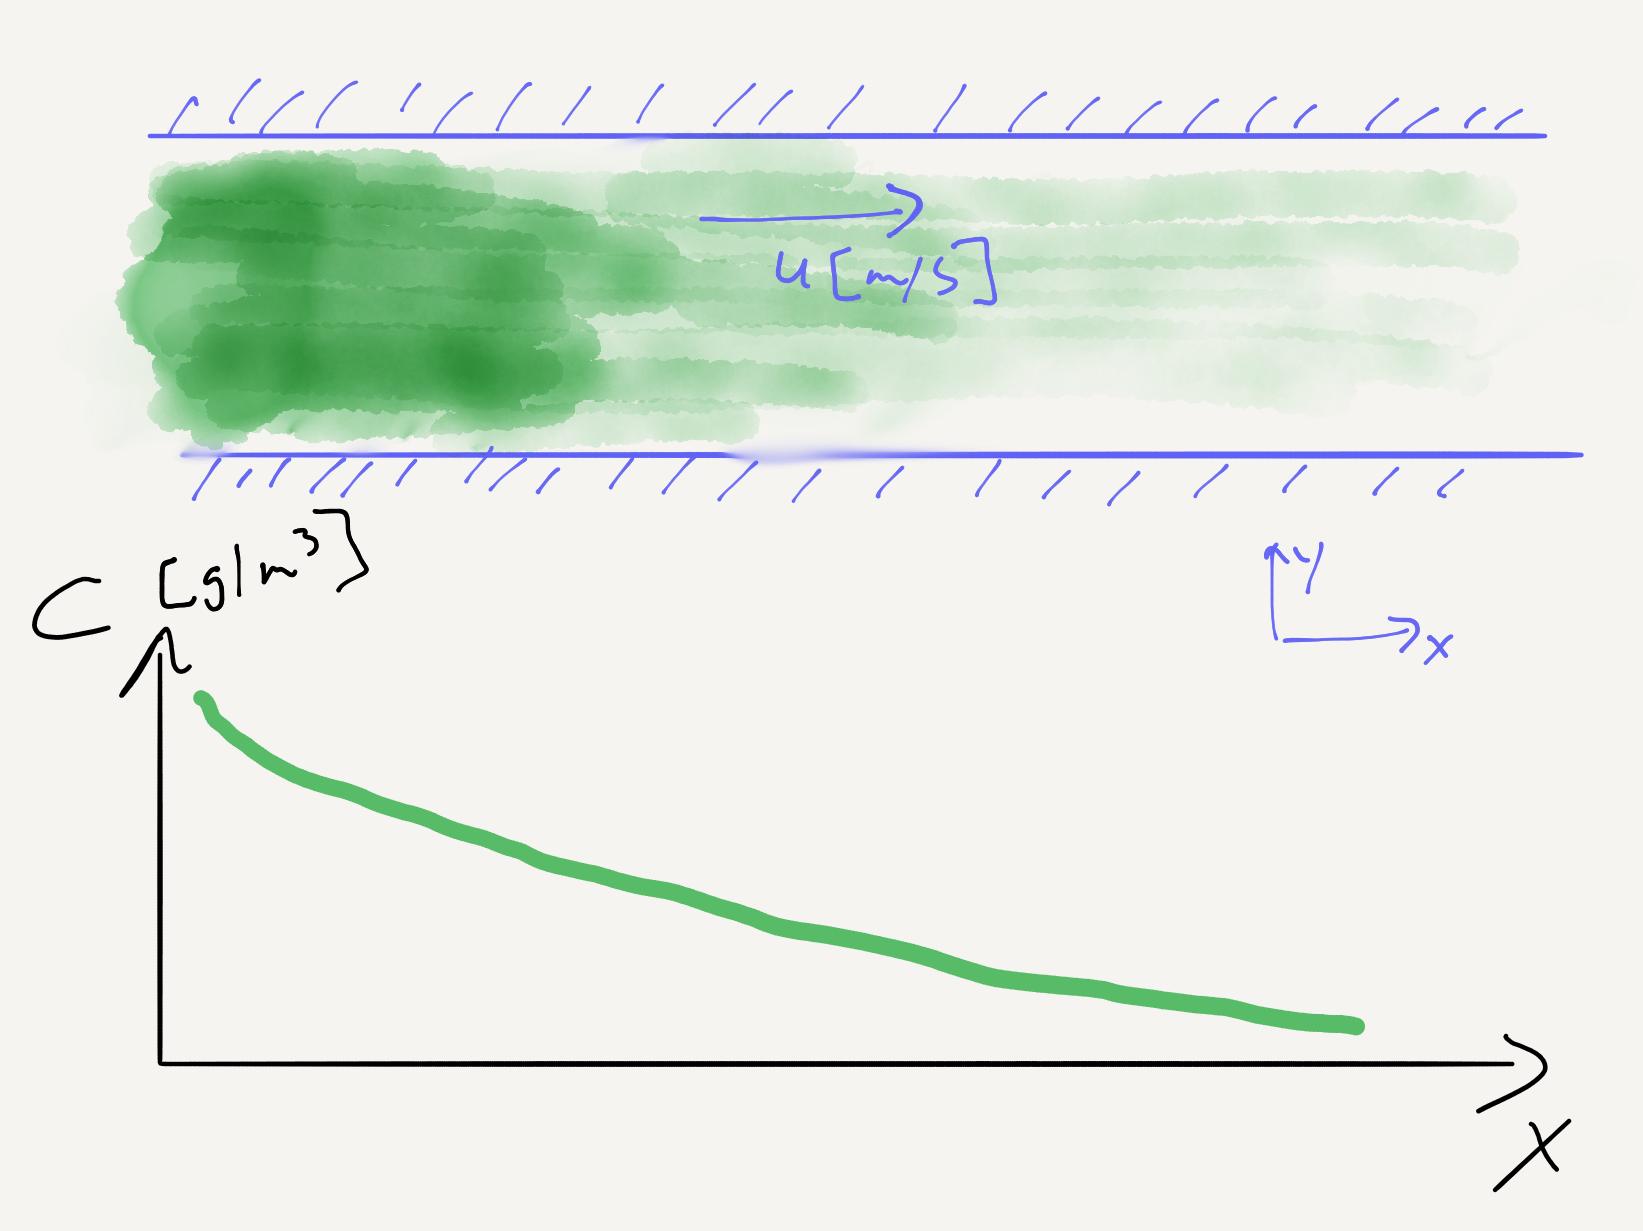
\includegraphics[width=2.5in]{FluxesFigs/ConcentrationRiver}
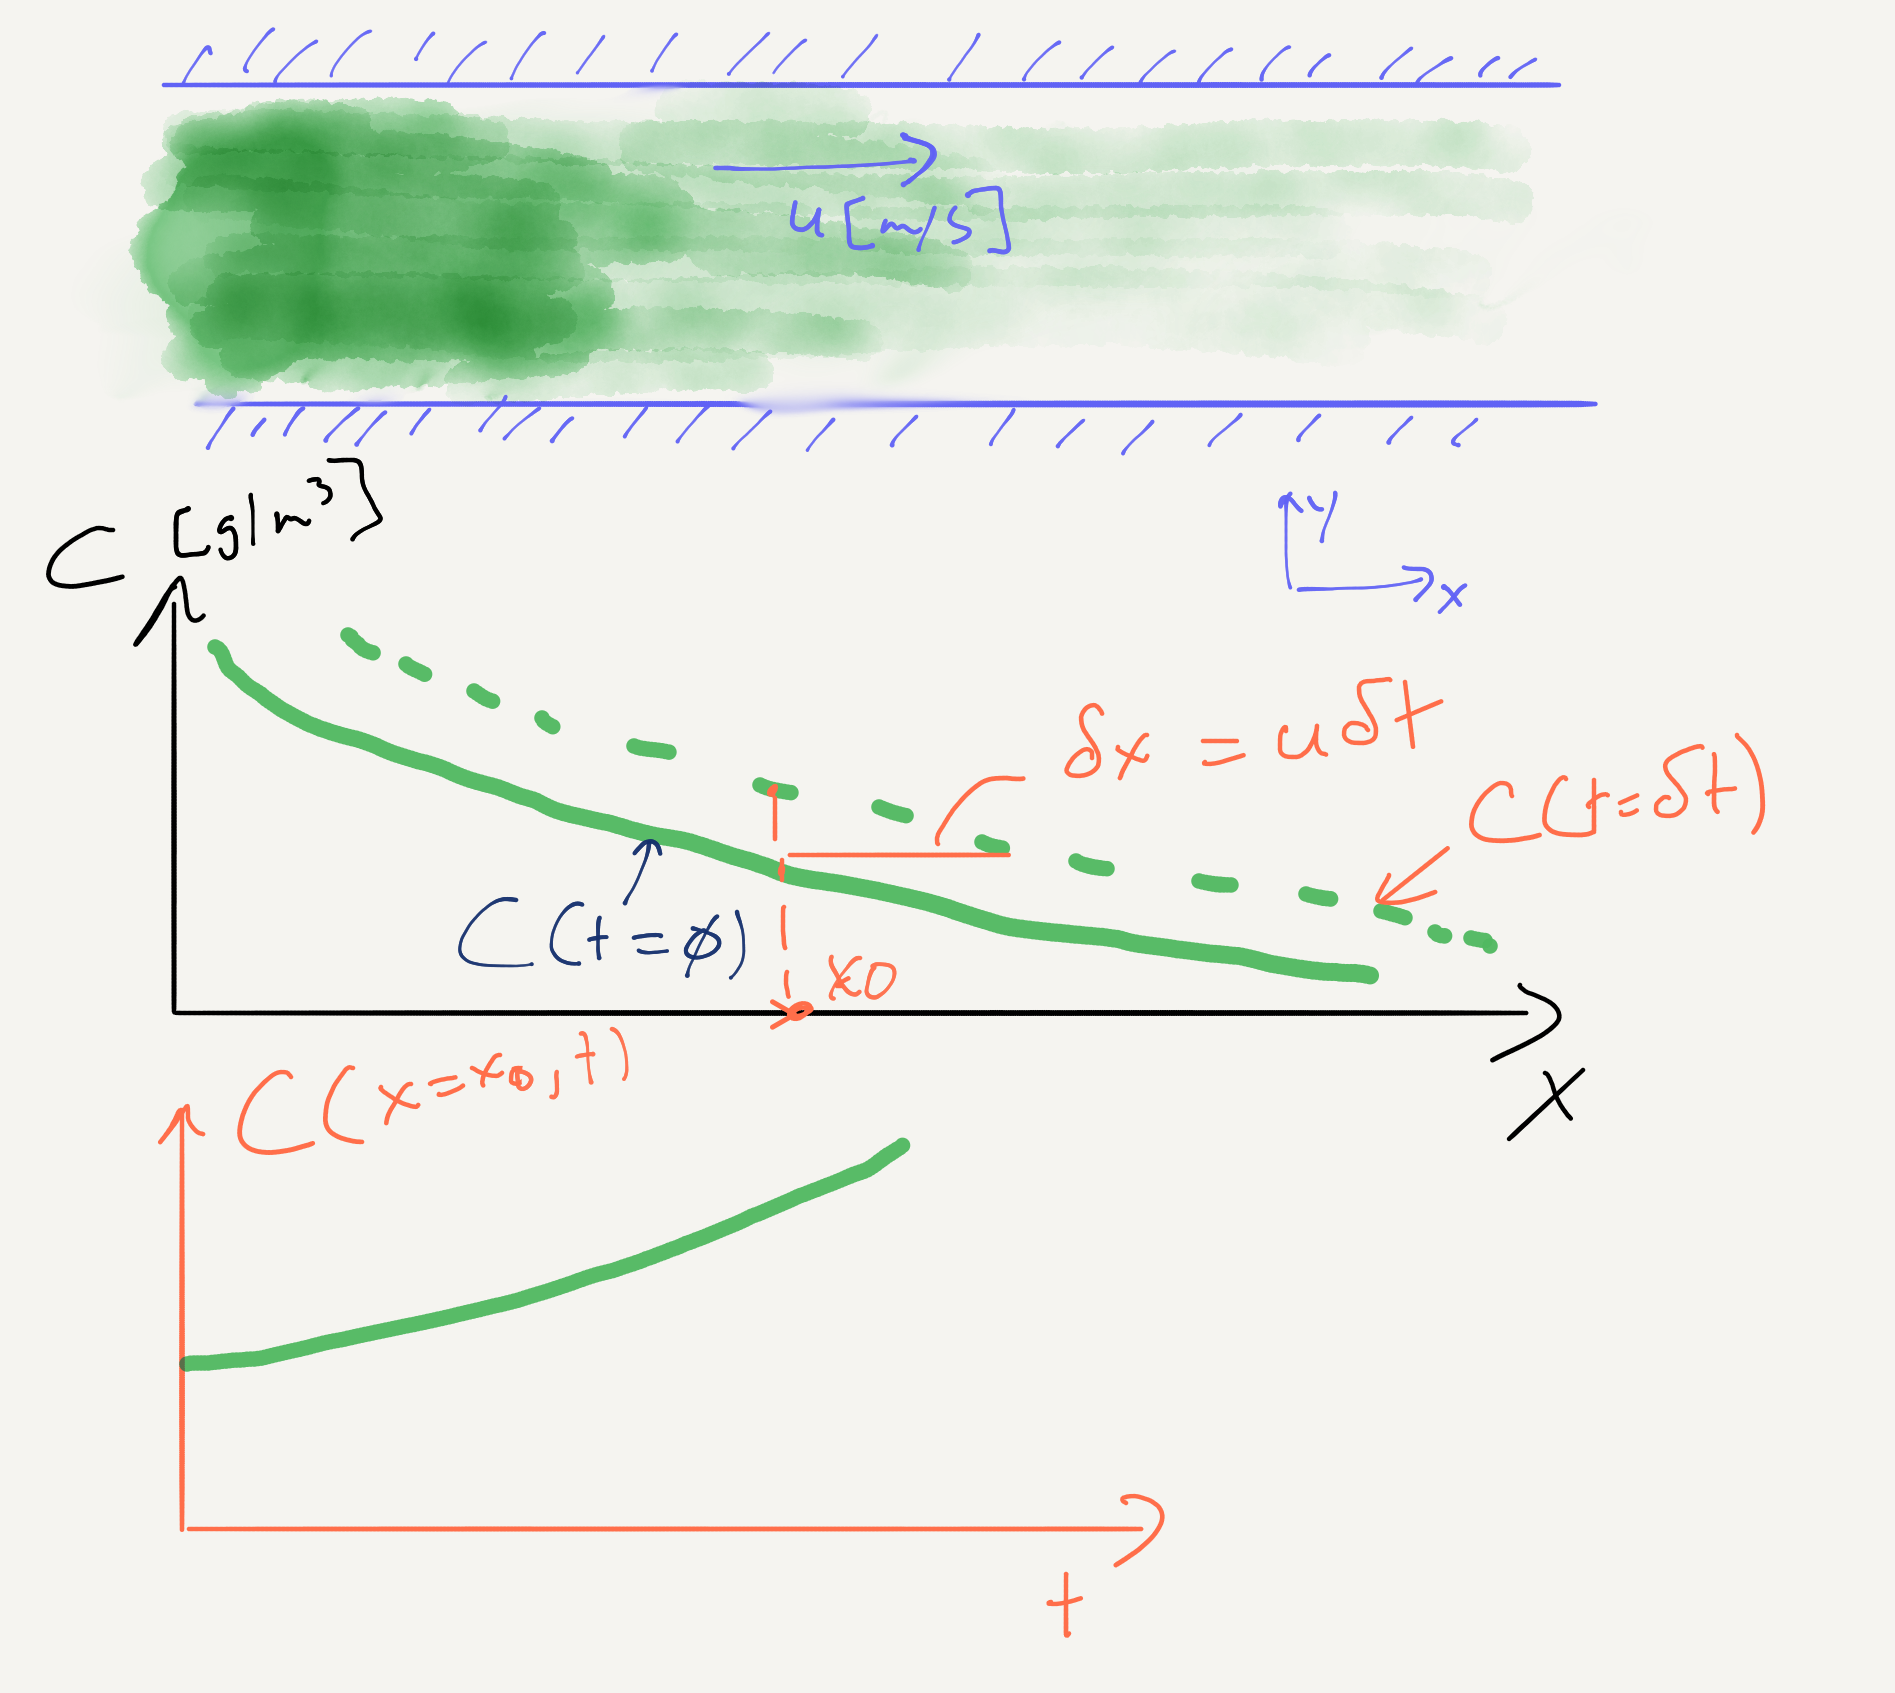
\includegraphics[width=2.5in]{FluxesFigs/ConcentrationRiverTime}
 \caption{Sketch of a river with a gradient of a contaminant.}
  \label{fig:ConcentrationRiver}
\end{center}
\end{marginfigure}


Advective fluxes are changes carried by gradients in the fluid.  So, imagine a river with a contaminant $C$ in it, measured with units of $\mathrm{g\,m^{-3}}$ (\fref{fig:ConcentrationRiver}), and the river is seen to have higher concentrations of contaminant upstream than downstream.    The river flows to the right with a speed $u\ \mathrm{[m\,s^{-1}]}$.   If we stand at some point on the river bank, say $x = x_0$, and measure the concentration over time, clearly, the concentration will be seen to be increasing.  Hopefully it is also clear that it is increasing at a rate that depends on how strong the gradient is and how fast the flow is.  If there were no gradient, then the concentration at $x_0$ would be constant, whereas if the gradient is strong the change will be faster.  

We can easily quantify this if we know the gradient of $C$ with $x$, $dC/dx$ and the speed of the river $u$.  At $x=x_0$, the concentration at a time $t=\delta t$ is
$C(t=\delta t) \approx C(t=0) - \delta x \frac{dC}{dx}$, where the approximation is very good so long as $dC/dx$ doesn't change much over the distance $\delta x$.  Here $\delta x$ is just the distance the river has travelled in time $\delta t$, and is therefore given by $\delta x = u \delta t$.  So we can predict the new concentration based on things we can measure as  $C(t=\delta t) \approx C(t=0) - u\ \delta t \frac{dC}{dx}$.  We allow $\delta t$ to become very small then we can write this as a differential:
\begin{equation}
\frac{dC}{dt} = -u \frac{dC}{dx} + \mathrm{other\ directions} + \mathrm{diffusive\ fluxes}    
\end{equation}
Note the minus sign, which accords with the sketch in \fref{fig:ConcentrationRiver} where $dC/dx < 0$ because the concentration decreases in the positive x direction.  

The term $-u\frac{dC}{dx}$ is the \emph{advective flux} in the x-direction.  Note that it has units of $\mathrm{g m^{-2}s^{-1}}$ and can be thought of as mass per time per area of the flow.   We can think of a river as only having one spatial dimension, but if there is more than one direction that can have gradients, as is often the case in the ocean, we may also be interested in the flux in the y-direction ($-v\frac{dC}{dy}$) and the vertical ($-w\frac{dC}{dz}$).  

\subsection{Advective transport} 

Note the units of an advective \emph{flux} are concentration per time (in this case $\mathrm{g m^{-3} s^{-1}}$).  However, now imagine we have a lake that the river is flowing into, and we want to know how quickly the total amount of contaminant in the lake is increasing or decreasing.  In this case we want the amount of contaminant per time that the river is carrying into the lake (i.e.\ in units of $\mathrm{g\, s^{-1}}$). In this case, we need to know not only how fast the river is moving, but also what its cross-sectional area is to get an \emph{advective transport} via:
\begin{equation}
    F_C = -u\ \delta A\ C \ \ \ \mathrm{[g\,s^{-1}]}
\end{equation} 
The term $Q = u\ \delta A$ is a volume transport, and usually has units of $\mathrm{ m^3\ s^{-1}}$.  

\subsection{Conservation of mass (and heat)}

Transports get used to create mass balance equations.  Since we know mass must be conserved (plus or minus releasing nuclear energy), the rate of change of the mass of a contaminant in a volume of water must be equal to the net transports of the contaminant into the volume.  A simple situation is to imagine a lake with two rivers, one feeding the lake and one draining it.  Suppose we measure the cross sectional area of the river, and the velocity to get $Q_{in}$, and that we measure the concentration of a contaminant in the river to be $C_{in}$.  Suppose the river that drains the lake does so at the same rate ($Q_{out} = Q_{in}$) and the concentration is $C_{out}$.  Then the rate of change of mass in the lake is simply:
\begin{equation}
    \frac{d M_C}{dt} = Q_{in} C_{in} - Q_{out}C_{out}
\end{equation}
where again, the rate of change is in $g/s$.  Sometimes we want to express this as a rate of change of the average concentration in the lake $\overline{C}_{lake}$ (where the overline emphasizes a volume average), in which case we would write as 
\begin{equation}
    \frac{d}{dt}\left(\overline{C}_{lake} V\right) = Q_{in} C_{in} - Q_{out}C_{out},
\end{equation}
where $V$ is the volume of the lake. If indeed $Q_{in} = Q_{out}$ then $V$ is a constant and 
\begin{equation}
    V\frac{d}{dt} \overline{C}_{lake}= Q_{in} \left(C_{in} - C_{out}\right).  
\end{equation}

The conservation of heat is very similar to the conservation of mass of a contaminant, but if the temperature range is not too large we can assume the heat capacity of water, $c_p$, is constant and think of this as the conservation of temperature:
\begin{equation}
    \frac{d}{dt}\left(\rho c_p \overline{T}_{lake} V\right) = Q_{in} T_{in}\rho_{in} c_p - Q_{out}T_{out} \rho_{out} c_p
\end{equation}
or if we assume density doesn't change very much with temperature we get an equation for temperature:
\begin{equation}
    \frac{d}{dt}\left(\overline{T}_{lake} V\right) \approx Q_{in} T_{in} - Q_{out}T_{out} 
\end{equation}
which we lazily call the "heat" equation.  

The conservation of salt is just the same as any other contaminant, but again, we just have to be careful of units.  Salinity is parts per thousand, so to get weight per volume, we need to multiply by the density of the water to get a mass equation:
\begin{equation}
    \frac{d}{dt}\left(\rho \overline{S}_{lake} V\right) \approx \rho_{in} Q_{in} S_{in} - \rho_{out}Q_{out}S_{out} 
\end{equation}
but again we just drop the density to get:
\begin{equation}
    \frac{d}{dt}\left(\overline{S}_{lake} V\right) \approx Q_{in} S_{in} - Q_{out}S_{out} 
\end{equation}

\begin{marginfigure}
    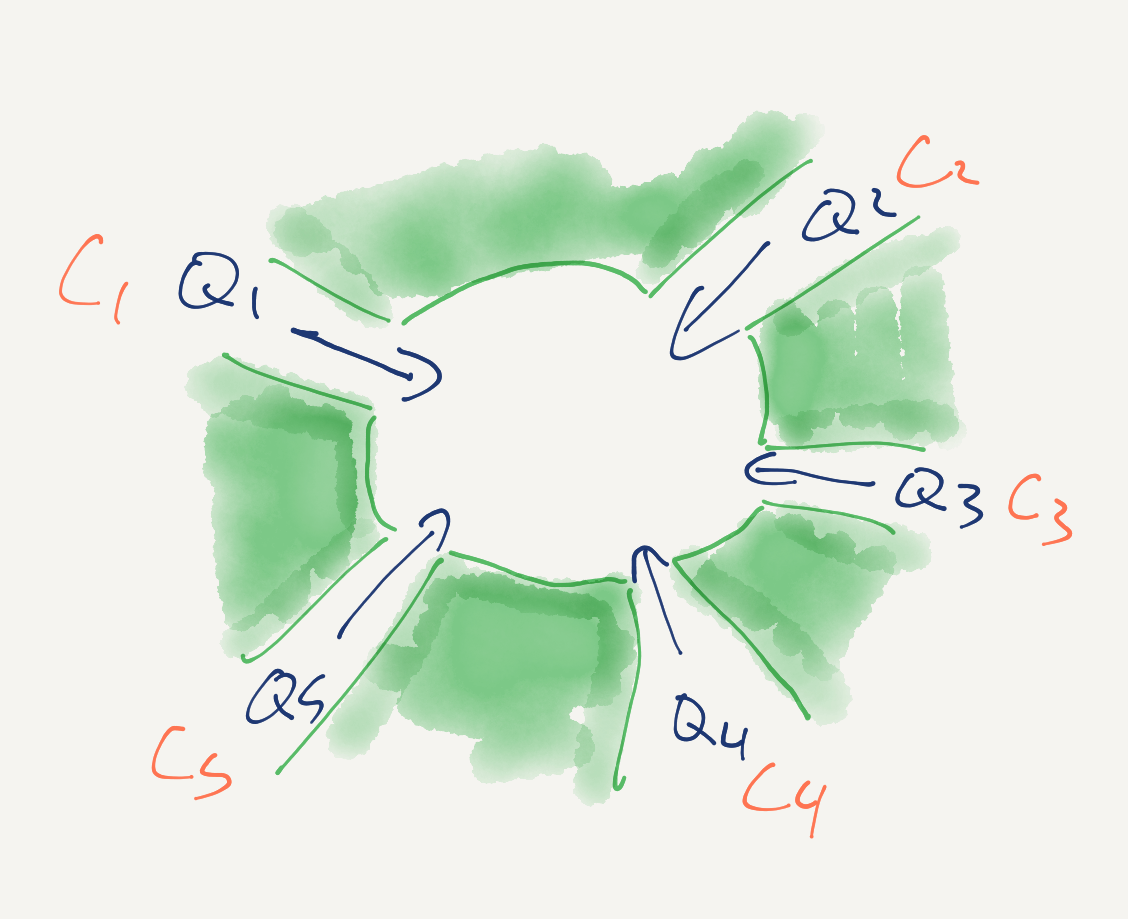
\includegraphics[width=2.5in]{FluxesFigs/SchematicLake}
    \caption{Schematic of lake with 5 possible inlets.  If $Q_i<0$ that means the flow is out of the lake.   }
\end{marginfigure}

The general form of all these equations is written as the rate of change of concentration in a fixed volume is equal to net sum of the inputs and outputs, so generally:
\begin{equation}
    \label{eq:sumMassCon}
    \frac{d}{dt}\left(C V\right) = \sum_{i=1}^N Q_{i} C_{i}
\end{equation}
where the sign of $Q_i$ is chosen to be positive into the volume, and negative if the flow is out of the volume.  



\begin{derivbox}[label={box:volumeintegral}]{Vector form of \fref{eq:sumMassCon}}
    If you have had vector calculus, then \fref{eq:sumMassCon} is equivalent to 
    \begin{equation}
        \frac{d}{dt}\int_V C \mathrm{d}V = - \oint_A C \mathbf{u}\cdot \mathrm{d}\mathbf{A},
    \end{equation} 
    where $\mathrm{d}\mathbf{A}$ is defined as positive pointing out of the volume.  The volume integral is the same as the finite sum as we make more and more finite sums.  
\end{derivbox}

\begin{marginfigure}
    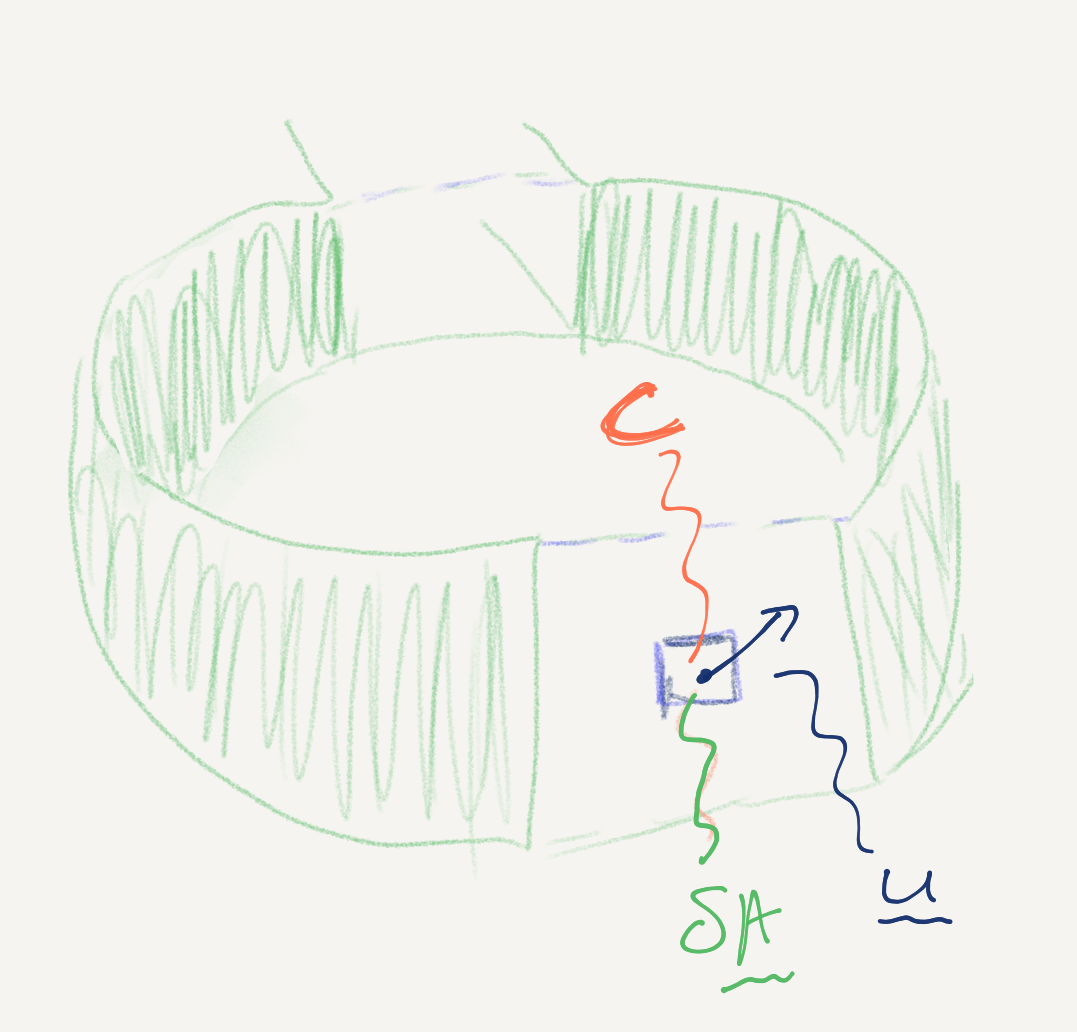
\includegraphics[width=2.5in]{FluxesFigs/SchematicVolumeIntegral}
    \caption{Schematic of volume integral.  The total integral is the sum of all ``open'' faces of the area that bounds the lake (i.e. you can only have fluxes out the open sides of the lake).}
\end{marginfigure}






\subsection{Conservation of mass and volume}

This application of the conservation of mass can be applied to the mass of water as well, but here we usually make a crucial approximation called that the fluid obeys \Wikiref{Incompressible flow}, and that variations of density are small enough to ignore in the mass equation.  This may seem counter intuitive, but it arises because the density of water does not vary much through the world's oceans (\fref{chap:EquationOfState}). 

For the mass of water, the conservation equation for our two-river lake is 
\begin{equation}
    \frac{dM}{dt} = Q_{in}\rho_{in} - Q_{out}\rho_{out}  \ \ \ \ \ \mathrm{\left[kg\ s^{-1}\right]}
\end{equation}
where $\rho_{in}$ and $\rho_{out}$ are the inflowing and outflowing density of the water in the lake.  Suppose also that $\overline{\rho}_{lake}$ is the average density in the lake, then we can write
\begin{equation}
    \frac{d}{dt}\left(\overline{\rho}_{lake} V \right) = Q_{in}\rho_{in} - Q_{out}\rho_{out}  \ \ \ \ \ \mathrm{\left[kg\ s^{-1}\right]}
    \label{eq:Mass}
\end{equation}
At a fundamental level, the incompressible flow approximation just says that $\overline{\rho}_{lake} \approx \rho_{in} \approx \rho_{out}$ and we can write
\begin{equation}
    \frac{d}{dt} V  \approx Q_{in} - Q_{out}  \ \ \ \ \ \mathrm{\left[m^{3}\ s^{-1}\right]}
    \label{eq:Volume}
\end{equation}
A little more justification is given in \fref{box:volume}, but assuming incompressibility of the fluid makes the mathematics significantly easier.  Of course one can always be more precise if needed.  


\begin{derivbox}[label={box:volume}]{More justification for dropping $\rho$}

    To see why its a good approximation to drop the density from the mass equation and just conserve volume, lets say that $\rho_{in} = \overline{\rho} + \rho'_{1}$ and $\rho_{out} = \overline{\rho} + \rho'_{2}$.  
    More formally, we can expand \fref{eq:Mass} using the chain rule:
    
    \begin{equation}
        V\frac{d}{dt}\left(\overline{\rho} \right) + \overline{\rho} \frac{d}{dt}\left(V\right) = \overline{\rho}Q_{in} - \overline{\rho}Q_{out} + \rho'_{1} Q_{in} - \rho'_{2} Q_{out}
    \end{equation}
    or, dividing by $\overline{\rho}$:
    \begin{equation}
        V\frac{1}{\overline{\rho}}\frac{d}{dt}\left(\overline{\rho} \right) + \frac{d}{dt}\left(V\right) = Q_{in} - Q_{out} + \frac{\rho'_{1}}{\overline{\rho}} Q_{in} - \frac{\rho'_{2}}{\overline{\rho}} Q_{out}
    \end{equation}
    A very large density variation in the ocean would be 1\%, so all the terms multiplied by $\frac{1}{\rho}$ are on order of 1\% of the terms that have not been multiplied by this factor.  Given that 1\% would be a very good estimate of any of the other terms, in a volume budget we usually ignore the small error and use \fref{eq:Volume}.  
    
    As an example, suppose $Q_{in} = 1\times10^{4}\ \mathrm{m^3\,s^{-1}}$ and $\rho_{in}=1000\ \mathrm{kg\,m^{-3}}$, and  $Q_{out} = 1.1\times10^{4}$ and $\rho_{out} = 1005$, and $\overline{\rho} = 1002.5$, and $V=10^{10}\ \mathrm{m^3}$.  We see that the terms are 
    \begin{equation}
    \frac{1}{\overline{\rho}}\frac{dM}{dt} = 10^{3} + 2.5 \ \ \mathrm{m^3\,s^{-1}}   
    \end{equation}
and that the second term is far smaller than the first.  

Getting at the left-hand term is actually a bit of work and requires an equation of state (\fref{chap:EquationofState}).  The density in the lake changes because of temperature or salinity changes in the body of water from the river.  This will give us $V\frac{1}{\rho}\frac{d}{dt}\left(\overline{\rho}\right)$.  To make life simple, imagine a linear equation of state that depends only on temperature: $\rho = 1000 (1 + \alpha (T - T_0))$ where $\alpha = 2\times10^{-4}\ \mathrm{\left[^oC^{-1}\right]}$ is a thermal expansion co-efficient.  
\end{derivbox}


\section{Diffusive Fluxes}

The other way that the concentration of a contaminant can change in a fluid is for the concentration to diffuse (or heat, or momentum).  The diffusion of a contaminant is at the molecular level due to the random motion of the particles in solution (\fref{fig:SchematicDiffusion}) which acts to homogenize the concentration of the contaminant.  This means that the flux of contaminant ($\mathrm{g m^{-2}s^{-1}}$) is from high concentration to low concentration.    Note that diffusive fluxes have exactly the same units as advective fluxes, and have the same effect on the concentration of the contaminant.  

\begin{figure}[hbt]
  \begin{center}
    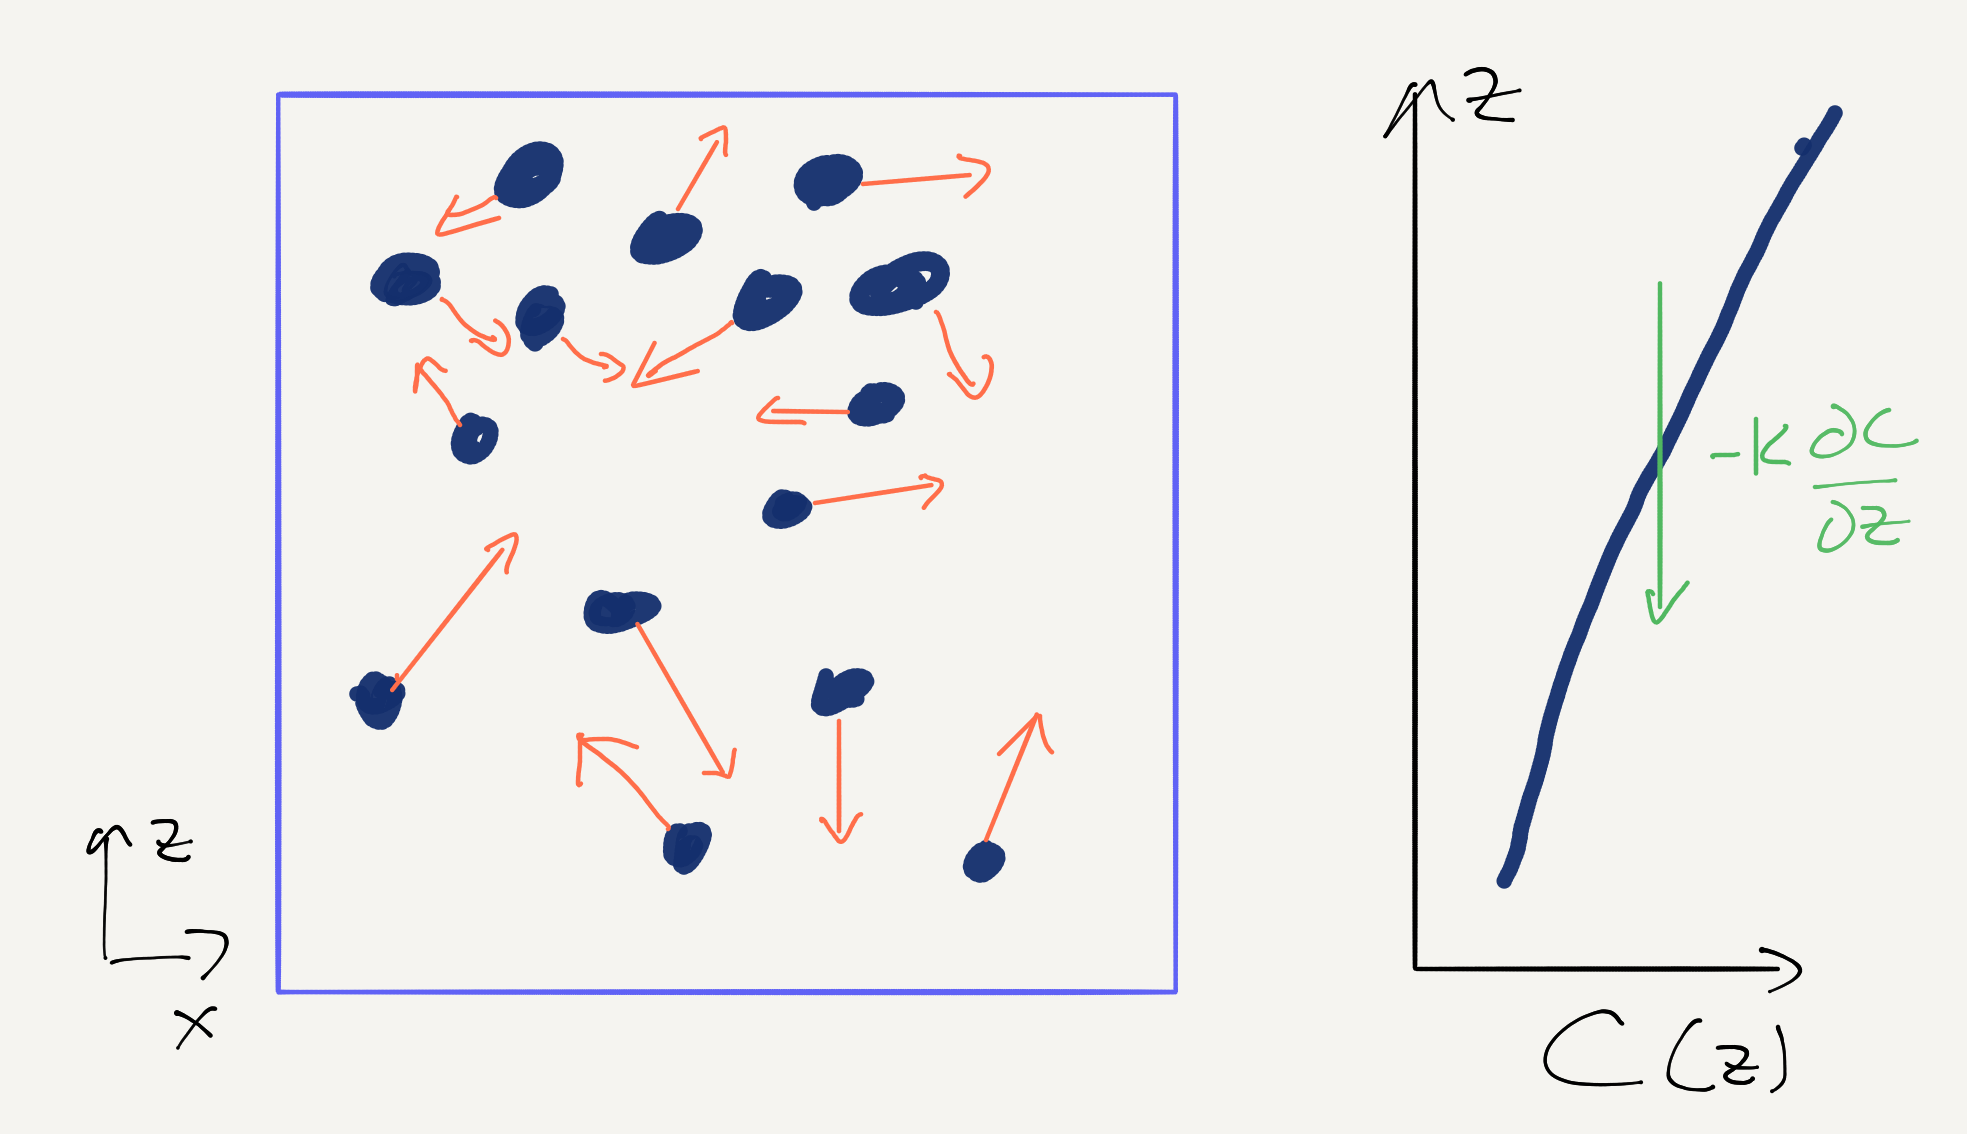
\includegraphics[width=4in]{FluxesFigs/SchematicDiffusion}
    \caption{Schematic of diffusion of a contaminant.  Random motions in the fluid act to homogenize the concentration, with a flux from high concentration to low concentration. }
    \label{fig:SchematicDiffusion}  
  \end{center}
\end{figure}

Most contaminants in fluids are assumed to obey \emph{Fick's Law} where the diffusive flux is linearly proportional to the gradient in concentration.  i.e. if there is a sharp change in the concentration, the flux is stronger.  And of course the flux is always from high concentration to low concentration, so we need a minus sign:
\begin{equation}
    \label{eq:Ficks}
    F = -K_C \frac{dC}{dz}
\end{equation}
where $K_C$ is the \emph{diffusion co-efficient}, and has units of $\mathrm{m^2\,s^{-1}}$. The sign of this flux indicates whether the flux is in the positive z-direction, or the negative.  So in \fref{fig:SchematicDiffusion}b, the $dC/dz > 0$ so the net diffusive flux of $C$ is downwards.  

The Diffusion co-efficient $K$ varies by the contaminant, or if temperature or momentum are being considered.  For salinity $K\sim 10^{-9} \ \mathrm{m^2\,s^{-1}}$, where the exact co-efficient depends on the salinity and temperature of the water.  For temperature, it is two orders of magnitude larger $K\sim 10^{-7}\ \mathrm{m^2\,s^{-1}}$, because the transfer of heat does not require molecules to trade position, but rather for vibrational energy (heat) to be transferred, which is a more efficient process.  

Of course, if we have a two- or three-dimensional distribution of the contaminant, then we need to consider the gradients in each direction.  i.e. going back to the example of the river, the diffusive flux would be in the same direction as flow, since the high concentration is coming from upstream, so in this case the flux is $-K dC/dx$.  

\section{Net flux: advection plus diffusion}

So, let us go back to considering how to determine how quickly the concentration changes at a given point in a fluid (\fref{fig:BothFluxesSchem}) by looking at a box in our river.  There is a flux from up stream ($F_L$) and one going downstream ($F_R$), so the net flux is $F_L - F_R$.  The rate of change is then given by 
\begin{equation}
    \delta x\, W\, H  \frac{d C}{d t} = \left(F_L - F_R\right) W H
\end{equation}, where $W$ is the width of the channel, and $H$ the depth, and 
 allowing $\delta x \to 0$
\begin{equation}
 \frac{d C}{d t} = -\frac{d F}{d x}
\end{equation}
So, if $F_L>F_R$ the concentration will increase in the volume.  

\begin{marginfigure}
  \begin{center}
    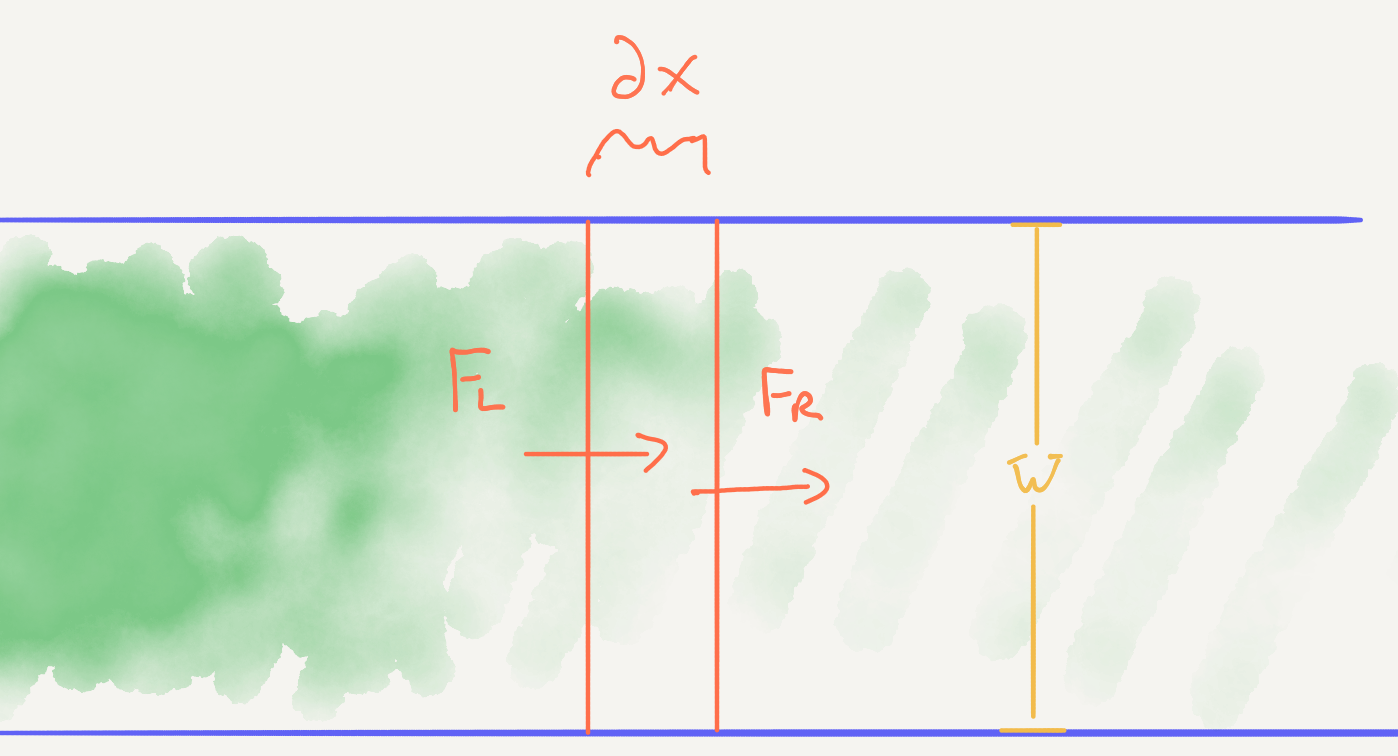
\includegraphics[width=2.5in]{FluxesFigs/BothFluxesSchem}
    \caption{Schematic of net flux into a small volume.}
    \label{fig:BothFluxesSchem}  
  \end{center}
\end{marginfigure}

At any given point, the flux in the x-direction is given by the advective plus the diffusive flux $F = uC - K \frac{dC}{dx}$, and the full conservation of mass is given by:
\begin{equation}
    \label{massboth}
    \frac{dC}{dt} = -u \frac{dC}{dx} + K \frac{d^2C}{dx^2} + \mathrm{other\ directions}
\end{equation}
Again, as discussed above, we can also think of this by considering the sum of fluxes across a number of inlets and outlets, but now with both advective and diffusive fluxes:
\begin{equation}
    \label{eq:sumMassConBoth}
    \frac{d}{dt}\left(C V\right) = \sum_{i=1}^N F_i = \sum_{i=1}^N \left( Q_i C_i - A_i K \frac{dC}{dn}\right)
\end{equation}
where $A_i$ is the area element the flux is passing through, and $dC/dn$ is a gradient, defined as positive into the volume.  

\begin{marginfigure}
    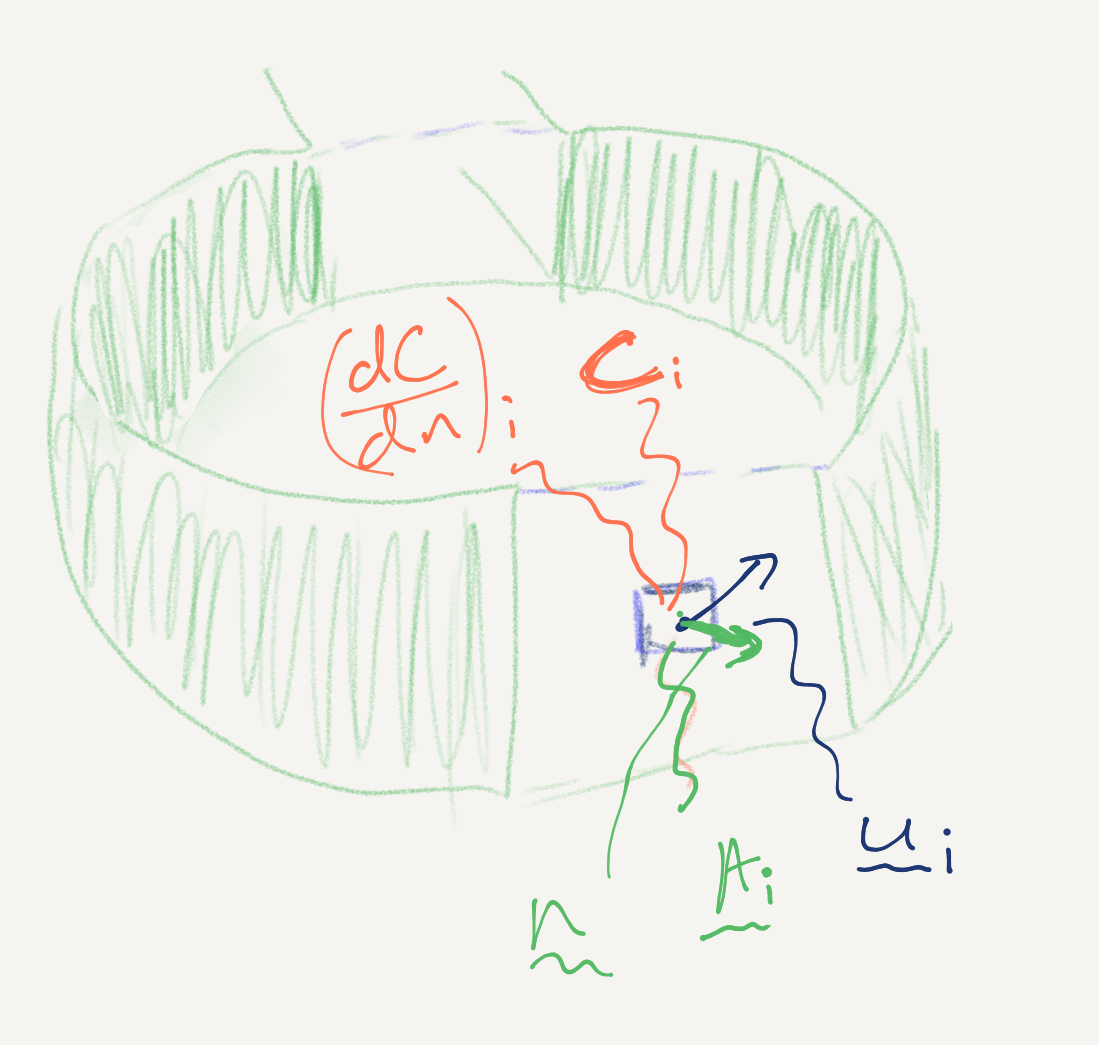
\includegraphics[width=2.5in]{FluxesFigs/SchematicLakeBoth}
    \caption{Information needed for mass budget across a surface leading out of a lake.}
\end{marginfigure}

Finally given these two types of fluxes, its possible for a gradient of a property to exist in the ocean and a mean flow, if the mean flow is balanced by diffusion.  Imagine if the river in \fref{fig:BothFluxesSchem} were flowing from right to left, then the advective flux would be to the left and the diffusive flux would be to the right, and it would be possible for the two fluxes to be in balance, and the concentration of contaminant to not change.  

\begin{derivbox}[label={box:volumeintegralboth}]{Vector form of \fref{eq:sumMassConBoth}}
Again, if we know a little vector calculus, we can rewrite \fref{eq:sumMassConBoth} as 
   \begin{equation}
        \frac{d}{dt}\int_V C \mathrm{d}V = - \oint_A \left(C \mathbf{u} - K\nabla C\right)\cdot \mathrm{d}\mathbf{A},
    \end{equation} 
where $C\mathbf{u}$ is the advective flux, and $-K\nabla C$ is the diffusive flux, both of which are vector quantities.  
\end{derivbox}

\subsection{Turbulent diffusivities}

\marginnote{\textsc{Time scale of diffusion}}

Molecular diffusion can be quite slow.  The diffusion equation ($\frac{dC}{dt} = -K \frac{d^2 C}{dx^2}$) can be solved with exponential functions (see \fref{box:exponentials}) that represent how quickly the solution relaxes to its steady state.  E.g. in \fref{fig:SketchDiffusionTime}, the temperature is fixed at two ends of an iron bar, and the initial temperature is cold, then heat will diffuse from the warm side to the cold side until a steady state is reached.  In this case, the steady state is a linear temperature gradient so that $d^2 T/dx^2 = 0$.  How quickly this will happen is given by the exponential approach to the steady state.

\begin{figure}[hbt]
  \begin{center}
    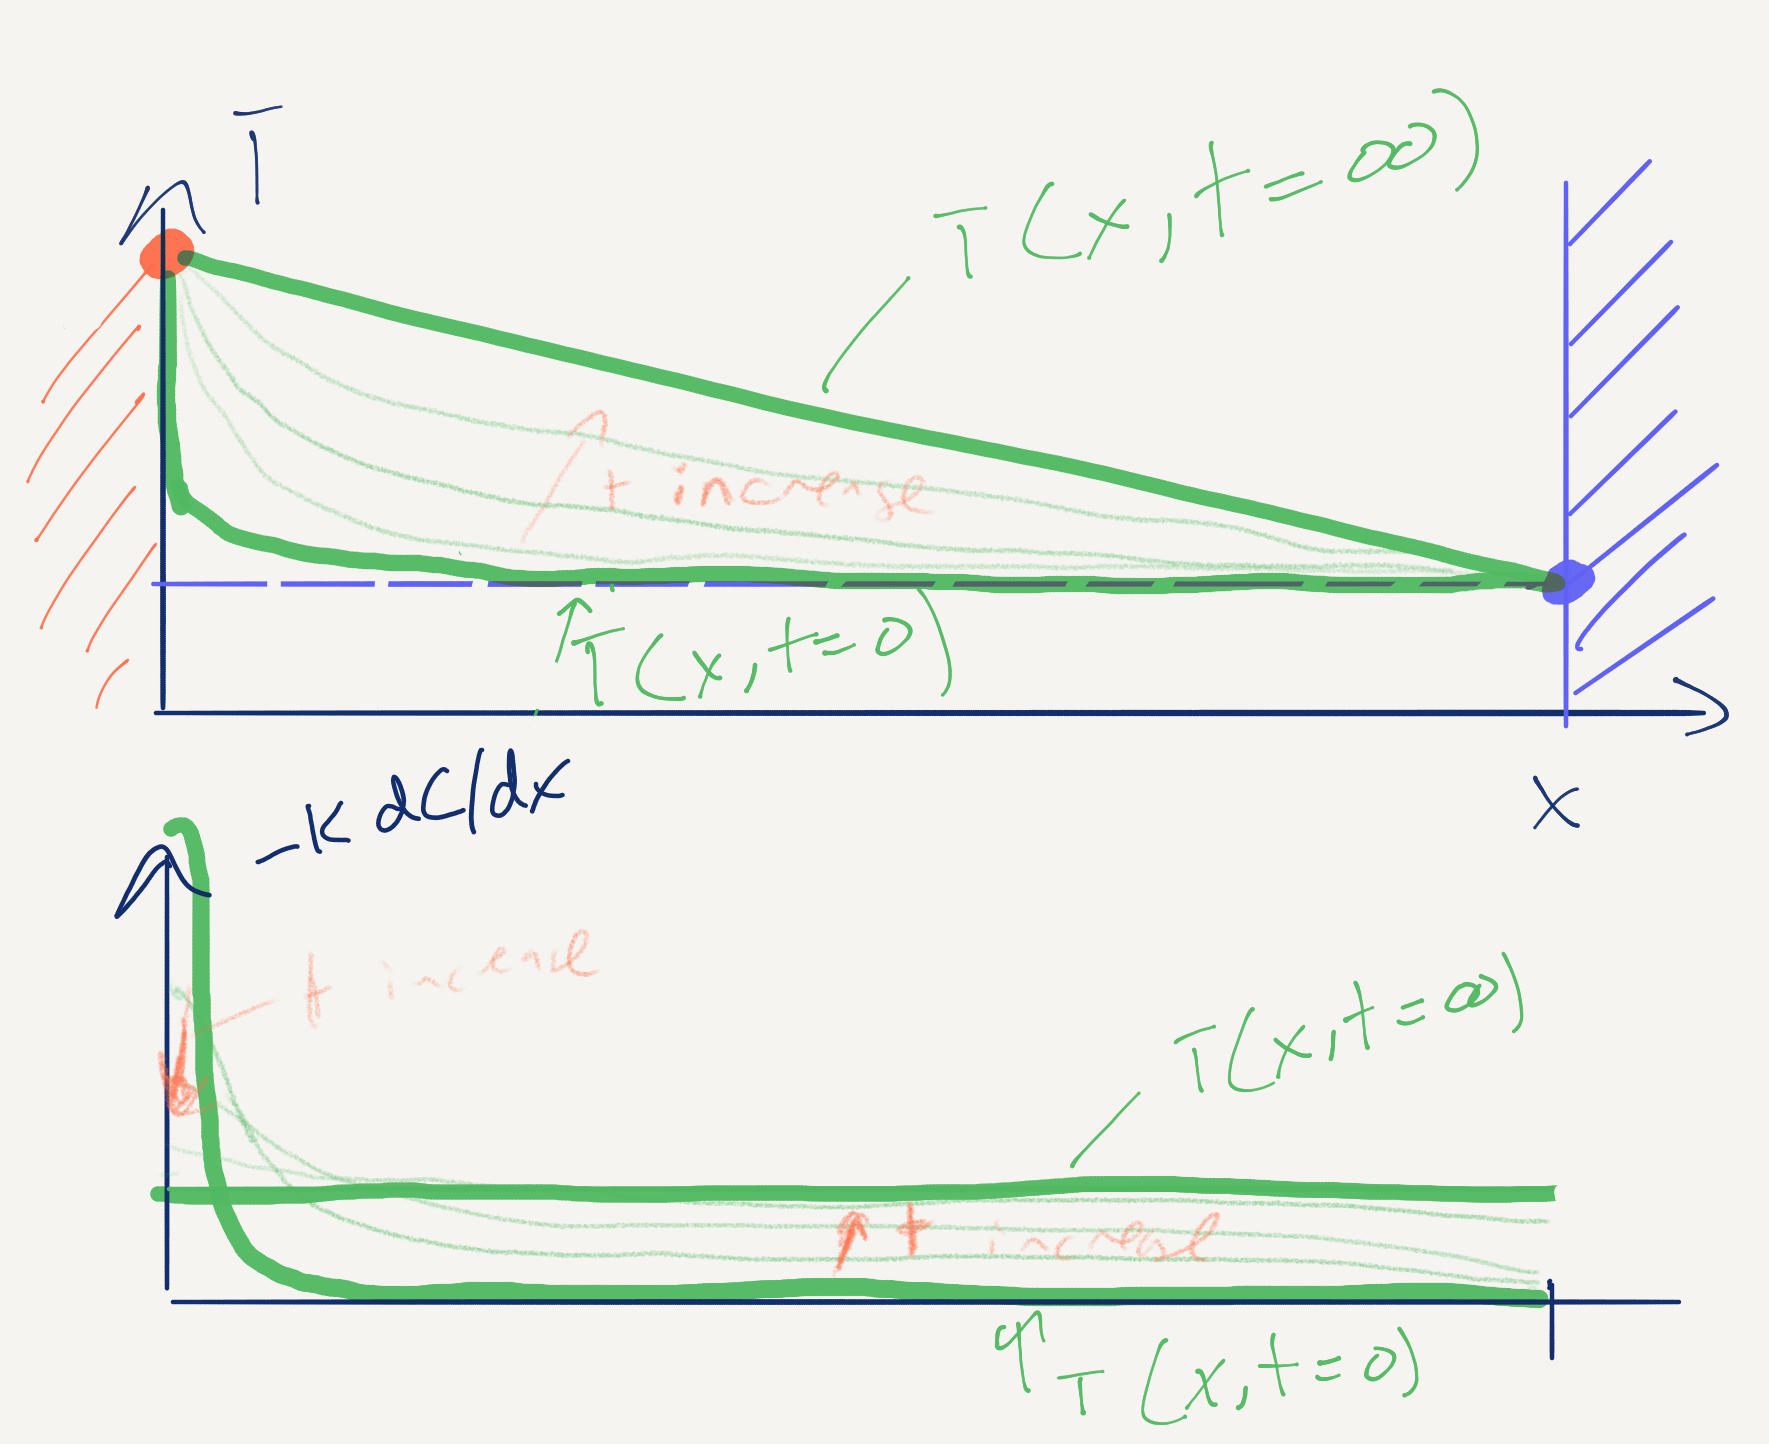
\includegraphics[width=3in]{FluxesFigs/SketchDiffusionTime}
    \caption{Example diffusion where temperature is fixed on the left and right side of the domain and the temperature all starts out cold.  Imagine an iron bar, with one end in a fire and the other end in a pool of water.  Heat diffuses in the bar from hot to  cold.  The steady state is a straight line between the two temperatures.}
    \label{fig:SketchDiffusionTime}  
  \end{center}
\end{figure}

We can estimate this exponential timescale, quite simply as $\mathcal{T} = L^2/K$, where $L$ is the spatial scale.  If we assume a 100-m lateral scale, and a molecular thermal diffusivity of $K=10^{-7}\ \mathrm{m^2\,s^{-1}}$, we would get a time scale of $10^{11}$ seconds, or more than 3000 years.  If we went all the way to the bottom of the 4000-m deep ocean, the time scale would be greater than 5 million years.  All these numbers are 100 times larger for salt.  

\begin{derivbox}[label={box:exponentials}]{Solutions to diffusion equation}
The diffusion equation $\frac{dC}{dt} = -K \frac{d^2 C}{dx^2}$ has solutions of exponential form:
\begin{equation}
    C = A e^{-K t/x^2} + B e^{K t / x^2} + C(x,t)
\end{equation}
where the values of $A$, $B$, and the function $C(x,t)$ depend on the initial conditions and boundary conditions. 
\end{derivbox}

\subsection{Turbulent diffusion}

Clearly, if molecular diffusivity were the only way that diffusion happened, we would just ignore these fluxes.  But we saw in \fref{chap:Estuaries} that mixing was an essential ingredient to the circulation.  What happens in the real ocean is that the flow is often turbulent, and turbulence stirs the fluid, and greatly enhances the efficiency of the molecular diffusion.  This is easy to see when you add milk to coffee or tea - if you do not stir the coffee, then the milk will stay in a blob.  Net diffusion only happens where there are gradients in the concentration (\fref{fig:SketchDiffTurb}). Stirring the fluid greatly increase the length of the fluid over which there is a gradient, and often sharpens the gradients. This leads to much more mixing than if the fluid is not stirred.  

\begin{figure}[hbt]
  \begin{center}
    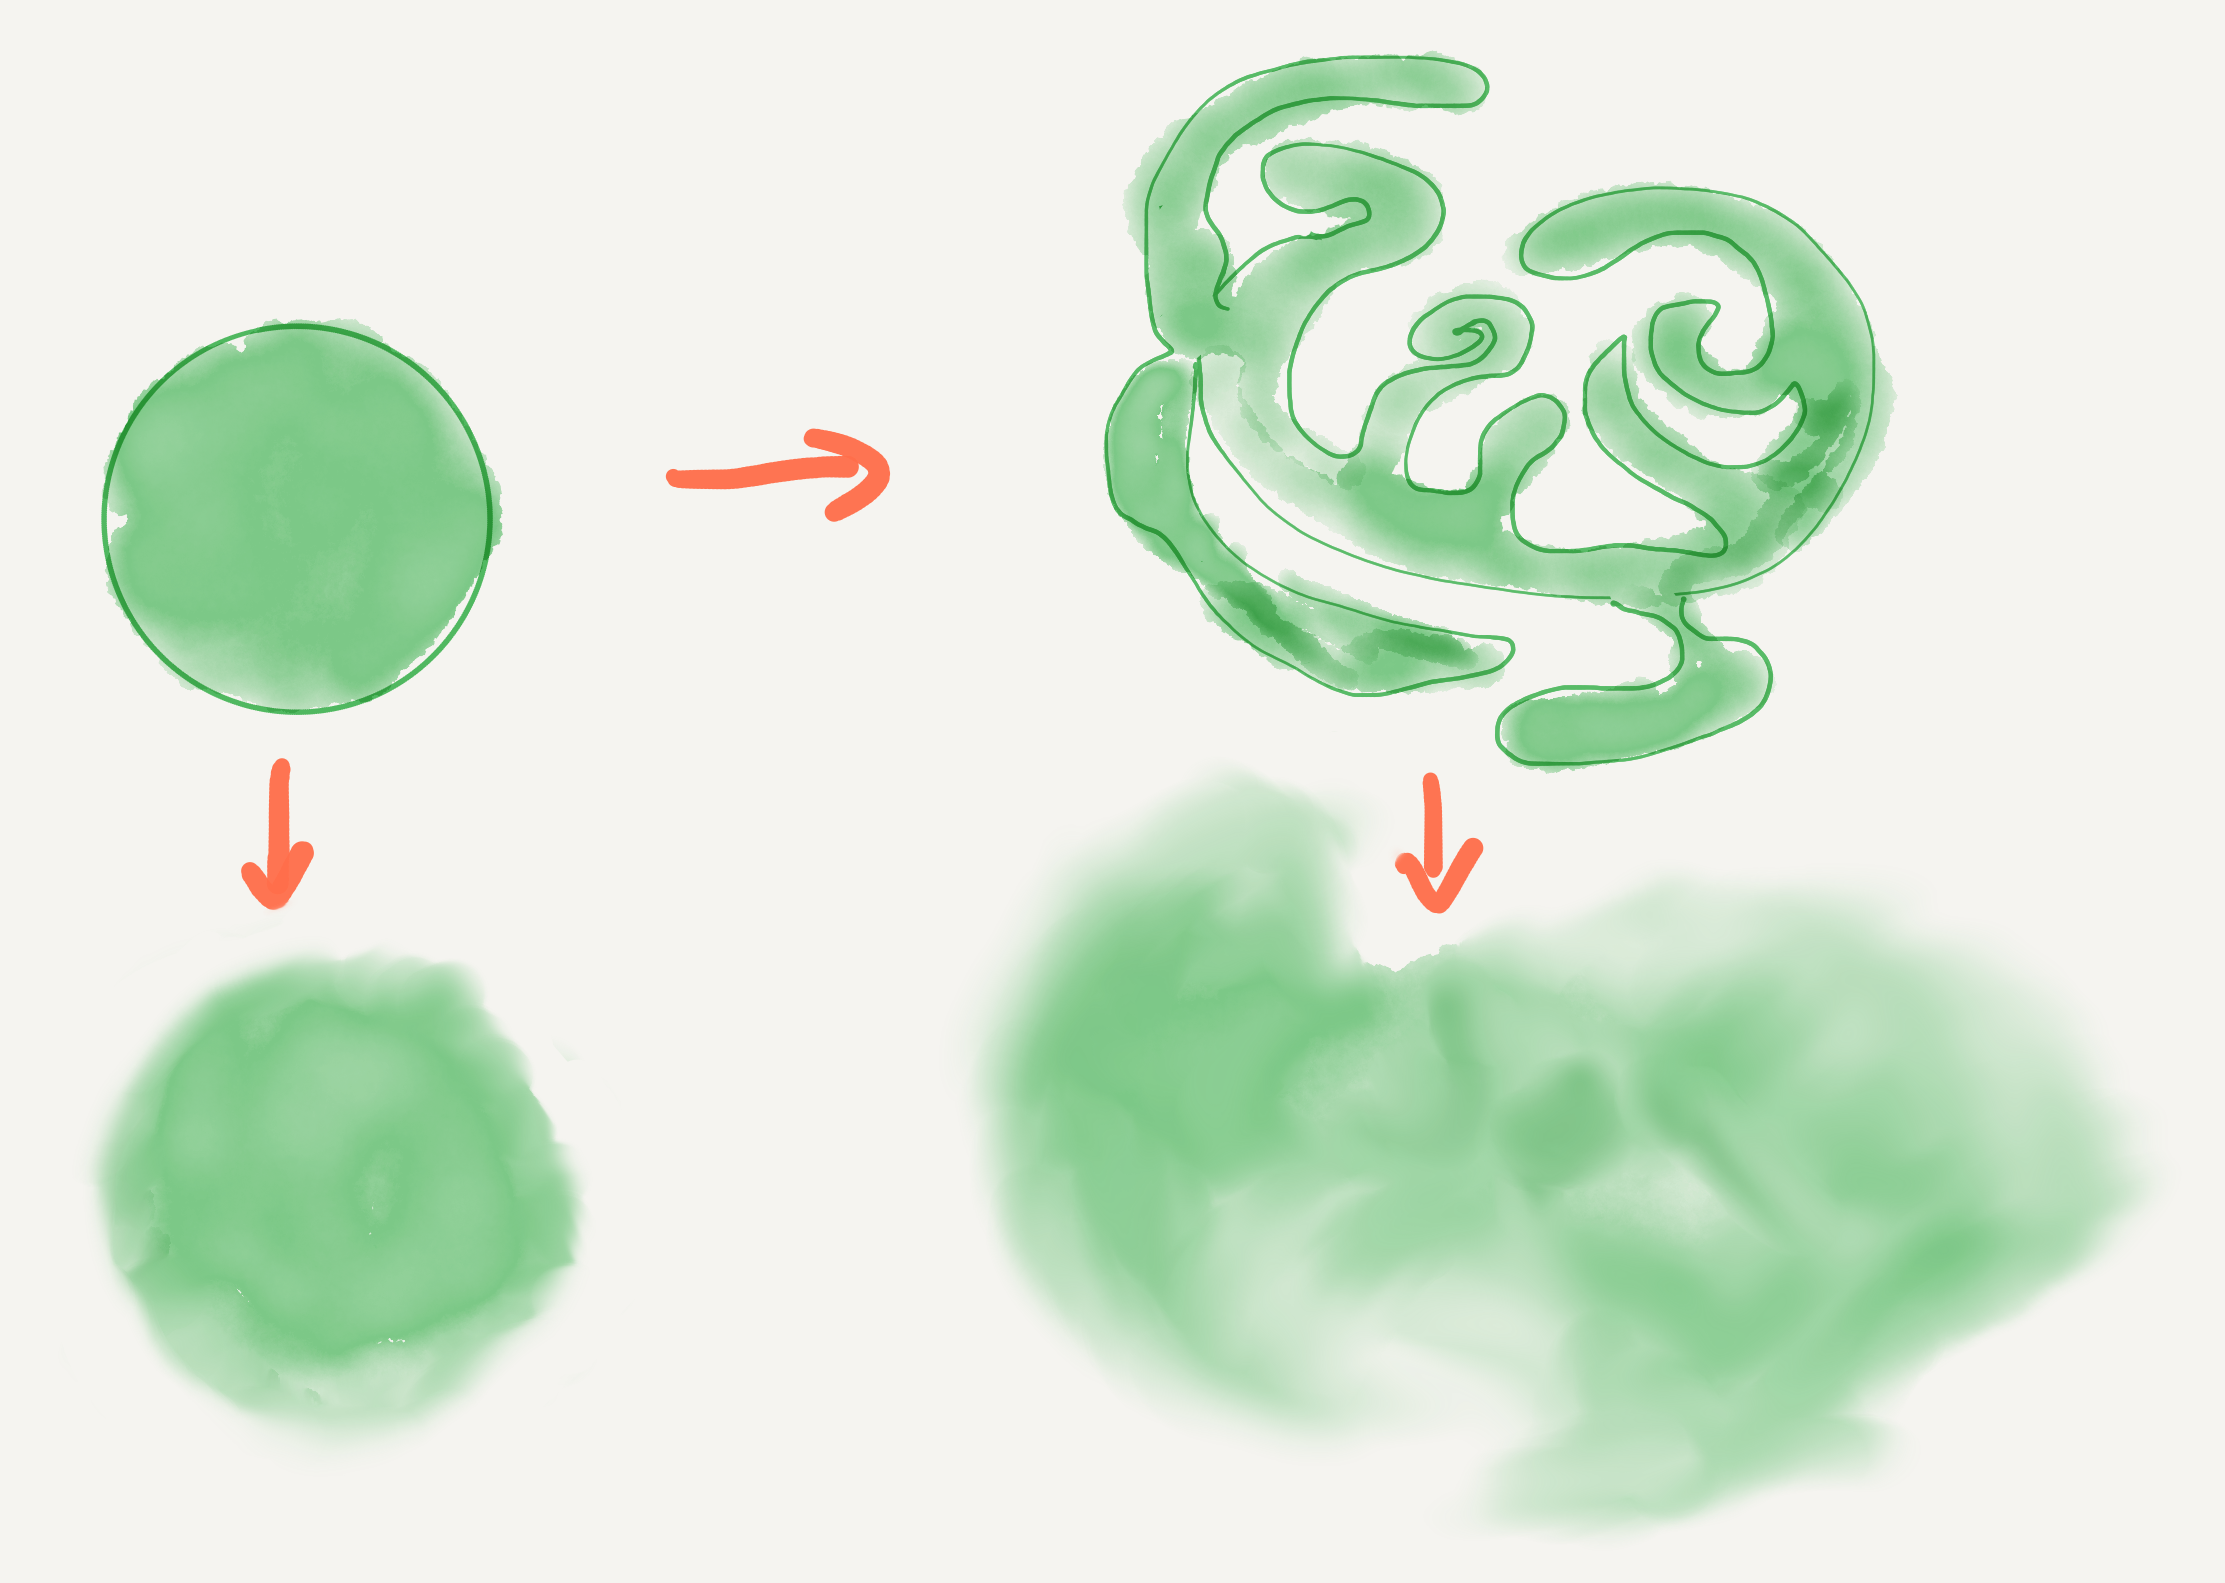
\includegraphics[width=3.5in]{./FluxesFigs/SketchDiffTurb}
    \caption{2-D sketch of the difference between diffusion and stirring and diffusion. Of course this happens in three dimensions in the ocean. }
    \label{fig:SketchDiffTurb}  
  \end{center}
\end{figure}

Stirring in the ocean is driven by a number of instability processes.  \emph{Shear instability} is one such process (\fref{fig:Smythetal05}) where the flow goes unstable because it has different velocities between layers.  In the simulation in \fref{fig:Smythetal05}, the instability grows and accomplishes significant stirring before it becomes fully three-dimensional turbulence which does more stirring.  The result is net mixing and thickened interface between the two layers.  A natural example from Admiralty inlet shows that this type of instability is often found in nature (\fref{fig:SeimGreggPlate2Trim}).  

\begin{figure}[hbt]
  \begin{center}
    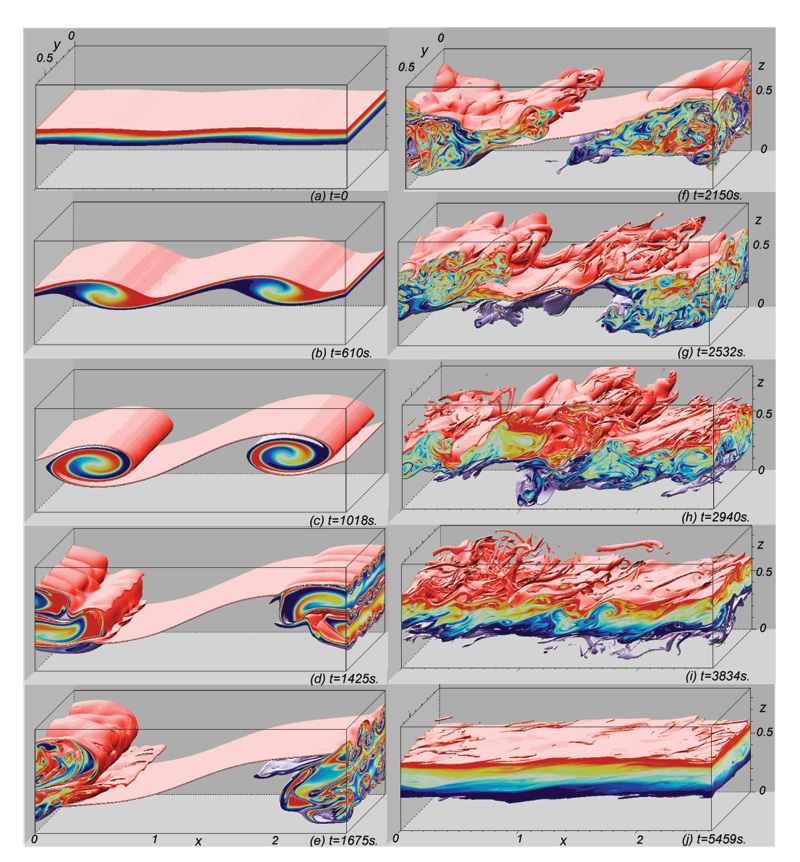
\includegraphics{./FluxesFigs/SmythEtAl05}
    \caption{Numerical simulation of mixing in the ocean.  Here a flow in the upper layer from left to right causes an instability on the temperature interface in the middle.  The flow breaks down into turbulence, and the turbulence stirs the fluid driving greatly enhanced mixing. \citep{smythetal05}}
    \label{fig:Smythetal05}  
  \end{center}
\end{figure}


\begin{figure}[hbt]
  \begin{center}
    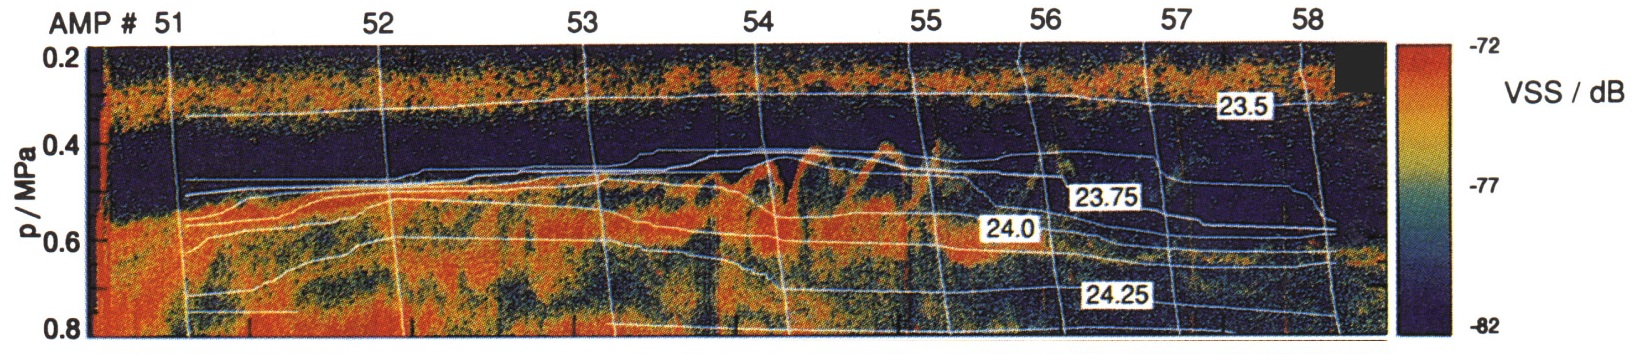
\includegraphics[width=4.5in]{FluxesFigs/SeimGreggPlate2Trim}
    \caption{Shear instability in the ocean measured at Admiralty Inlet in Puget Sound \citep{seimgregg94}. }
    \label{fig:SeimGreggPlate2Trim}  
  \end{center}
\end{figure}

A second common instability is \emph{convective instability}.  This happens when dense fluid is on top of light fluid, such as happens when you boil water on the stove.  A more oceanographic experiment is shown in \fref{fig:ConvectionANU} where the water is warmed from below.  As it rises, there is clear instabilities, however note that these instabilities themselves are actually shear instabilities when looked at closely.  

\begin{figure}[hbt]
  \begin{center}
    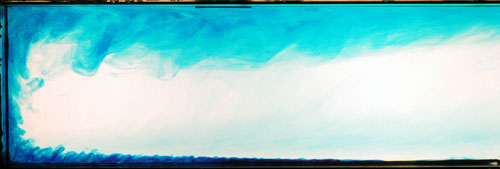
\includegraphics[width=4.5in]{FluxesFigs/ConvectionANU}
    \caption{Horizontal convection experiment where the left side of a tank is heated at the bottom, and the right hand side (not shown) is cooled.  Water rises, primarily along the left hand wall.  \url{http://rses.anu.edu.au/gfd/AR2005/index.php?p=ar05res}}
    \label{fig:ConvectionANU}
  \end{center}
\end{figure}

The effect of turbulence is to greatly increase the rate at which properties are fluxed across interfaces.  However the flux still tends to be from regions of high concentration to regions of low concentration.  Hence we will often represent these fluxes by a linear flux law.  For instance, in the x-direction: $F_x = -K \frac{dC}{dx}$ where now $K$ is a \emph{turbulent diffusivity} rather than a molecular one.  When estimated, turbulent diffusivities are \emph{much} larger than molecular diffusivities.  Estimates in the open ocean range from molecular levels to $K\sim 10^{-1}\ \mathrm{m^2s^{-1}}$ and levels can reach even higher values in coastal waters where there are strong flows.  Estimating turbulence requires sophisticated instrumentation and often simplifying models, and remains a great challenge today to oceanographers.  Often the approach to estimating turbulence is to relate the turbulence to external parameters that can be measured or simulated.  This has lead to many schemes to estimate turbulence in models and ocean calculations.  

The consequence of turbulent mixing is that it makes the importance of mixing much more apparent.  If the timescale is $10^{11}\ \mathrm{s}$ for molecular diffusion at $K=10^{-7}\ \mathrm{m^2\,s^{-1}}$, then it is $10^{7}\ \mathrm{s}$ for $K=10^{-3}\ \mathrm{m^2\,s^{-1}}$, or 100 days.  That starts to matter for long-lasting flows.  

%%% Local Variables:
%%% mode: latex
%%% TeX-master: t
%%% End:
